% This is a LaTeX thesis template for Monash University.
% to be used with Rmarkdown
% This template was produced by Rob Hyndman
% Version: 6 September 2016

\documentclass{monashthesis}
\usepackage{booktabs,caption}
\usepackage[flushleft]{threeparttable}
\usepackage{float}
\usepackage{amsmath}
\usepackage{bm}
\usepackage{rotating}

%%%%%%%%%%%%%%%%%%%%%%%%%%%%%%%%%%%%%%%%%%%%%%%%%%%%%%%%%%%%%%%
% Add any LaTeX packages and other preamble here if required
%%%%%%%%%%%%%%%%%%%%%%%%%%%%%%%%%%%%%%%%%%%%%%%%%%%%%%%%%%%%%%%

\author{Zhixiang Yang}
\title{Disaggregated Sectoral Employment Dynamics in Australia}
\studentid{30306396}
\def\degreetitle{Bachelor of Commerce (Honours)}
% Add subject and keywords below
\hypersetup{
     %pdfsubject={The Subject},
     %pdfkeywords={Some Keywords},
     pdfauthor={Zhixiang Yang},
     pdftitle={Disaggregated Sectoral Employment Dynamics in Australia},
     pdfproducer={Bookdown with LaTeX}
}


\bibliography{thesisrefs}

\begin{document}

\pagenumbering{roman}

\titlepage

{\setstretch{1.2}\sf\tighttoc\doublespacing}

\clearpage\pagenumbering{arabic}\setcounter{page}{0}

\hypertarget{acknowledgement}{%
\chapter*{Acknowledgement}\label{acknowledgement}}
\addcontentsline{toc}{chapter}{Acknowledgement}

I would like to express gratitude to my supervisor Professor Farshid Vahid and my coordinator Professor Heather M Anderson for their selfless support and devoted care along the way. I would also like to thank my family and Xiefei Li for their continuous supports and encouragement.

\vspace{48pt}

\texttt{Matlab\ version.\ 2022a} codes are used to generate the estimated coefficients for the proposed Bayesian VAR model.

R \texttt{4.1.2\ "Bird\ Hipple"} \autocite{R} and Rstudio \texttt{2022.07.1+554\ "Spotted\ Wakerobin"} \autocite{Rstudio} are used for data analysis in this thesis.

\vspace{12pt}

R package used and their versions in this research include \texttt{matrixStats\ 0.61.0} \autocite{package_matrixStats}, \texttt{ggplot2\ 3.3.5} \autocite{package_ggplot2}, \texttt{zoo\ 1.8.9} \autocite{zoo}, \texttt{tidyverse\ 1.3.1} \autocite{tidyverse}, \texttt{dplyr\ 1.0.8} \autocite{dplyr}, \texttt{stats\ 4.1.2} \autocite{stats}, \texttt{readr\ 2.1.2} \autocite{readr}, \texttt{pracma\ 2.3.8} \autocite{pracma}, \texttt{lubridate\ 1.8.0} \autocite{lubridate}, \texttt{fpp3\ 0.4.0} \autocite{fpp3}, \texttt{ggpubr\ 0.4.0}\autocite{ggpubr}, \texttt{ggrepel\ 0.9.1} \autocite{ggrepel}, \texttt{directlabels\ 2021.1.13} \autocite{directlabels}, \texttt{gghighlight\ 0.3.3} \autocite{gghighlight}.
(\emph{Note: In no particular order above})

\vspace{12pt}

This thesis is produced using the R package \texttt{bookdown\ 0.25} \autocite{bookdown} with the Rmarkdown template package \texttt{monash\ 0.0.0.9000} for the honours thesis in the Department of Econometrics and Business Statistics, Monash University \autocite{monash}

\hypertarget{declaration}{%
\chapter*{Declaration}\label{declaration}}
\addcontentsline{toc}{chapter}{Declaration}

I declare that this thesis contains no material which has been submitted in any form for the award of any other degree or diploma in any university or equivalent institution, and that, to the best of my knowledge and belief, this thesis contains no material previously published or written by another person, except where due reference is made in the text of the thesis.

\vspace{12pt}

-- Signature: \underline{\emph{\textbf{Elvis Zhixiang Yang}}}

\hypertarget{abstract}{%
\chapter*{Abstract}\label{abstract}}
\addcontentsline{toc}{chapter}{Abstract}

I investigate the performance of Australian employment at a disaggregated level and compare the post-COVID situation with the no-COVID situation. A multivariate time series model is utilised to determine the long run employment spillovers to total employment at the two-digit subsectoral level. My results suggest that in the two-digit subsectoral level, ``Other Store-Based Retailing'', followed by ``Administrative Services'', ``Furniture and Other Manufacturing'' will generate the strongest positive spillovers to the total economy. One of the main contributions of this paper is that the government can stimulate these high and positive spillovers to recover total employment effectively and efficiently. Moreover, I evaluate the impacts of COVID-19 on the Australian labour market with counterfactual analysis. The outcomes demonstrate that the pandemic has a long-lasting effect on the economy. In addition, I point out the main reason behind the lowest unemployment rate record and compare the no-COVID scenario for unemployment rate. The spillover analysis together with the evaluation, thus, provide another aspect for policymarkers to improve the Australian economy at the post-pandemic stage.

\hypertarget{the-australian-covid-19-pandemic-background}{%
\chapter{The Australian COVID-19 Pandemic Background}\label{the-australian-covid-19-pandemic-background}}

The COVID-19 pandemic has had a massive impact on global economies. Millions of workers have been furloughed or even fired across the globe as businesses struggled to survive \autocite{ny2020}. The same situation occurred in Australia, due to increased restrictions, many businesses closed their doors, while employees worked few hours or were laid off by businesses. As a result of the continued ``lockdown'' periods in 2020, the Australian Bureau of Statistics \autocite{ABS2021} estimated that 72\% of businesses generated less revenue and the underemployment rate reached a historical high of 13.8\% by the end of April, 2020, only one month after the outbreak of COVID-19.

Our research is motivated by the lack of quantitative research on the employment of two-digit disaggregated industry subsectors in Australia, despite the fact that many studies have focused on the aggregated employment rate. The loss of hierarchical information is a common issue with aggregated studies, which can lead to biased conclusions or the illusion of prosperity in the labour market. In this manner, a quantitative analysis of sectoral employment will alleviate this problem, allowing us to better assess the effects of COVID-19 in Australia.

\hypertarget{research-aim-and-questions}{%
\section{Research Aim and questions}\label{research-aim-and-questions}}

This research will expand on \textcite{anderson2020} by using data from 87 two-digit industry sectors rather than the 19 sectors that they used previously. I will develop a model for the two-digit subsectors to assess the long run effect and the COVID-19 post-impacts. In addition, I will present a counterfactual analysis based on the optimistic assumption that no COVID-19 or major events occurred. The two-digit sectoral data will provide us with more valuable information, allowing us to gain a deeper understanding of employment dynamics in Australia at a disaggregated level.

The overall goal of the research is to provide estimates of two-digit sectoral employment based on historical data. My specific objectives are as follows:

\begin{enumerate}
\def\labelenumi{\arabic{enumi}.}
\item
  Create a time series model of employment in 84 two-digit subsectors of the Australian economy.
\item
  To conduct a counterfactual analysis using this model.
\item
  To use this model to determine which two-digit subsectors have the highest long-term impact (or positive spillover) on employment growth in the long run.
\end{enumerate}

\hypertarget{thesis-structure}{%
\section{Thesis Structure}\label{thesis-structure}}

This thesis examines Australian Employment at a disaggregated level before estimating the long run effects of COVID-19 on the sectoral employment rate in Australia. The rest of the thesis is organised as follows. First, in chapter 2, I begin by reviewing the existing literature in the relevant fields. Second, in chapter 3, I will provide data sources as well as an exploratory data analysis. Then, in chapter 4, I will present our selected model. After we have chosen our model, I will conduct a counterfactual analysis to assess the impact of COVID-19 and provide useful insights on key beneficial industries after COVID-19 in chapter 5. Finally, in chapter 6, I will provide a brief conclusion and discuss the limitations and potential future extensions.

\clearpage

\hypertarget{review-of-literature}{%
\chapter{Review of literature}\label{review-of-literature}}

We focused our review of the existing literature on two major topics:

\begin{enumerate}
\def\labelenumi{\arabic{enumi}.}
\item
  The COVID-19 sectoral impacts and economic modelling
\item
  Bayesian VAR Modelling of large numbers of time series
\end{enumerate}

\hypertarget{sectoral-impact-of-covid-19.}{%
\section{Sectoral Impact of COVID-19.}\label{sectoral-impact-of-covid-19.}}

Most existing studies have concentrated on assessing the effects of COVID-19 on broad sectors of large economies such as the US and Europe. To predict the impacts of COVID-19, \textcite{ludvigson2020covid} developed a disaster series to translate the macroeconomic impact of costly and deadly disasters in recent US history and model them as sectoral shocks. They concluded that the shock would result in a cumulative loss of 20\% in industrial production, 39\% in public services and a 12.75 percent reduction in US GDP by the end of 2020. \textcite{gregory2020pandemic} conducted simulations under various scenarios via a search theoretic model using US data and discovered that the recovery in the U.S. would be L-shaped, with employment remaining lower than pre-covid for a long period. They also expanded the research to a disaggregated level of 20 sectors, predicting that the ``arts and entertainment'' and ``accommodation and food services'' sectors would experience the hardest hit during the pandemic.

In Australia, \textcite{anderson2020} developed a multivariate time series model for 19 main sectors (as a typical small open economy) using a Bayesian VARX model. According to their findings, ``Manufacturing'' and ``Construction'' have the greatest positive spillovers for the overall economy. Meanwhile, they also applied a ``conditional forecasting'' method proposed by \textcite{waggoner1999} to forecast different scenarios of total employment in Australia after the pandemic. However, their research did not use a finely disaggregated level in Australia (two-digit subsectors of main sectors), which may be less informative in macroeconomic analysis.

\hypertarget{baysian-var}{%
\section{Baysian VAR}\label{baysian-var}}

The Bayesian Vector Autoregression model (BVAR) is commonly used in the literature for high-dimensional multivariate modelling \autocites[e.g.][]{anderson2020,litterman1986,banbura2010large}. The BVAR model is appealing because it allows us to estimate a large number of parameters when the sample size is small, in a statistically coherent way. \autocite{litterman1986,wozniak2016bayesian}.

To utilize the Bayesian VAR estimators, \textcite{litterman1979} proposed the Minnesota Prior, which decreases the weight of the lagged variables with the lag length. The prior mean on the first own lag is set to unity and the rest are set to zero so that \emph{(a)} the most recent lag should provide more information than distant lags; and \emph{(b)} own lags should explain more than the lags of other variables.

\hypertarget{setting-minnesota-prior-with-shrinkage}{%
\section{Setting Minnesota Prior with Shrinkage}\label{setting-minnesota-prior-with-shrinkage}}

The literature suggests that a significant improvement in the predicting performance of large BVAR dynamic models can be made by more careful choice of the prior assumptions \autocite{banbura2010large,litterman1986}. Additionally, \textcite{robertson1999vector} and \textcite{kadiyala1997} proposed a Normal-inverse-Wishart prior to put the Minnesota prior in our estimated model, by preserving its main characteristics. Particularly, \textcite{banbura2010large} suggested incorporating dummy observations into the BVAR system as an easier way to apply the Normal-inverse-Wishart prior (see Appendix A for details).

\clearpage

\hypertarget{data-collection-and-exploratory-analysis}{%
\chapter{Data collection and exploratory analysis}\label{data-collection-and-exploratory-analysis}}

\hypertarget{data-introduction-and-wrangling}{%
\section{Data Introduction and wrangling}\label{data-introduction-and-wrangling}}

The data I use for this thesis comes from the Australia Bureau of Statistics (ABS), which covers 86 industry sub-divisions of main jobs. The ABS records the employment (measured in thousands of people \(('000)\)) from \(1984:Q4\) to \(2021:Q4\) with a structure shown in Figure \ref{fig:anzsic}.

\graphicspath{ {/Users/elvisyang/Desktop/hon_proj/Disaggregated_Employment/Honours_thesis/figures} }

\begin{figure}[H]
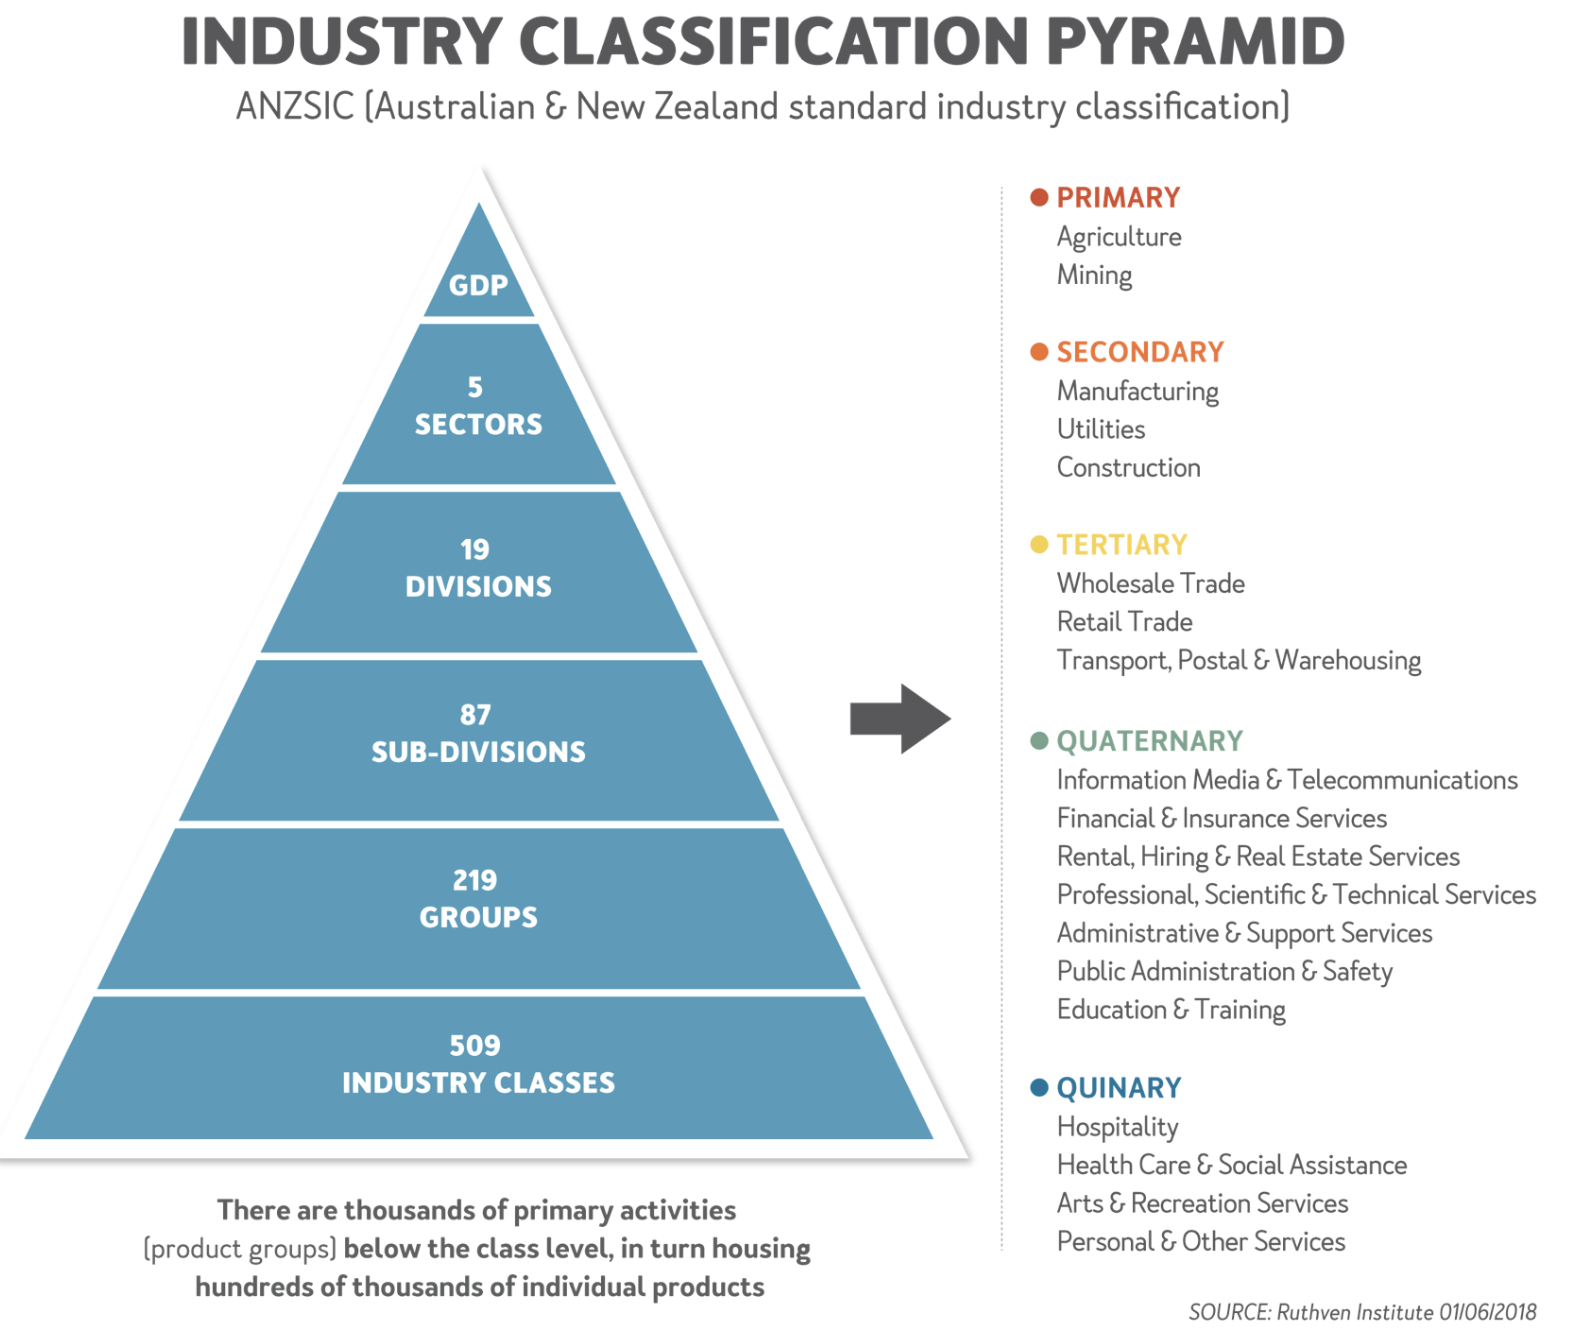
\includegraphics[scale=0.5]{ANZSIC}
\centering
\caption{Australian Industry Pamamid plot by (ANZSIC)}
\label{fig:anzsic}
\end{figure}

Although seasonally adjusted data is available in \autocite{ABS2022}, however, the seasonal adjustment of post-COVID data is problematic as shocks caused by lockdowns would affect the post-covid seasonality. In addition, the seasonally adjusted subsectoral data do not add up to total employment, which prevents the model from maintaining internal consistency (such as forecasting coherence) in the model. Therefore, rather than using the seasonally adjusted data provided by the Australian Bureau of Statistics, I use the original quarterly employment data with transformations (see description below) to capture any potential changes in seasonal patterns.

In this thesis, I only downloaded the data from the fourth quarter of 1984 to the second quarter of 2022. I also use Microsoft Excel to extract both the employment for two-digit disaggregated levels as well as total employment. It should be noted that some of the data are zero, which makes a log transformation impractical. As a result, I will make the changes below to get rid of them while preserving the coherence of the data structure. The cleaned data can be seen in the \emph{ABSemp.xlsx} file at (\url{https://github.com/elvisssyang/Disaggregated_Employment}).

\begin{itemize}
\item
  Merge the two-digit subsector \emph{57- Internet Publishing and Broadcasting} and \emph{54- Publishing (except internet)} to a new combined subsector called \emph{54 Publishing and broadcasting}.
\item
  Combine the \emph{96 Private Households Employing Staff and Undifferentiated Goods and Service Producing Activities of Households for Own Use} and \emph{95 Personal and Other Services} as \emph{95 Personal and other services (include activities for own use)}.
\end{itemize}

It is obvious that the ABS employment data contains few non-classified series (nfd). Because ABS offers no additional information, I will not discuss these series in this thesis. If this is incorporated into the model, it will have an impact on the sectoral dynamics. To make the forecasts coherent (sum to total employment) and analysis universal, I will not take them into account at this stage. As a result, my total employment data differs from the total employment data that has been published. The largest discrepancy, however, concerns only a small portion of the real total employment. Accordingly, this will not have a big impact on our analysis.

When there are no zeros, a log transformation can be used to explain the percentage change in employment. To generate accurate forecasts from the estimated VAR model, we need the data to be stationary. Thus, I will further apply a fourth difference (seasonal difference) to eliminate the seasonality and nonstationarity for the original quarterly data.

Finally, in \emph{Chapter 6}, I also combine the following data together with the number of employment by subsectors \autocite{ABS2022} to further support our counterfactual analysis:

\begin{itemize}
\item
  Total Labour Force: Downloaded from ABS website (see \textcite{ABS2022}) \footnote{This includes the number of employment by subsectors, which is the original data we use in this thesis.}.
\item
  Unemployment Rate: Downloaded from ABS website (see \textcite{ABS2022a})
\end{itemize}

\hypertarget{preliminary-exploratory-data-analysis}{%
\section{Preliminary Exploratory Data Analysis}\label{preliminary-exploratory-data-analysis}}

Figure \ref{fig:19} illustrates the changes in the raw data for 19 key sectors in Australia between 2010 and 2022. As a result of business closings and travel bans in 2020:Q2, we can observe that the number of total employment dropped substantially (from around 13,200,000 to 12,200,000 in \(2020:Q2\)). Figure \ref{fig:19} illustrates how most industries behaved similarly and underwent significant changes during the pandemic. The ``Accommodation \& Food'', ``Media \& telecom'' and ``Arts'' industries have experienced a severe loss of employment when compared to the previous data of these industries, and have not yet fully recovered to the pre-covid level. Some industries, such as ``Financial'' and ``Healthcare'', on the other hand, essentially remained the same as pre-COVID period and displayed an ongoing upward trend.

When compared to the sectoral level, the employment of subsectors at the two-digit level illustrates a different pattern (see Figure \ref{fig:86}). As shown in Figure \ref{fig:86}, the subsectors ``Food and Beverage Services'', ``Construction Services'', ``Professional, Scientific and Technical Services (Except Computer System Design and Related Services)'' and ``Other Store-Based retailing'' are relatively large subsectors with various losses. For example, the ``Food and Beverage Services'' subsector increased steadily from 2010 Q1 to 2020 Q1, but was significantly impacted by the first lockdown in 2020 Q2, which resulted in a loss of about 210,000 employed people. On the other hand, ``Construction Services'', which belongs to the construction sector, did not experience a sizable decline during the pandemic. Similar to the ``Professional, Scientific and Technical Services'' subsector, it recovered the loss in just two quarters and is expected to increase in the future.

However, only taking into account the 19 broad sectors has a disadvantage in that the two-digit subsectoral dynamics of these sectors might not be consistent with their aggregated sectoral changes. For instance, one might assume that the corresponding subsectors would exhibit the same pattern based on the aggregated performance of the ``Education'' and ``Healthcare'' sectors at the 19 sectoral level (see Figure \ref{fig:19}). However, the reality is that while there is an overall upward trend in the ``Healthcare'' sector or in the ``Education'' sector, some of their two-digit subsectors perform differently (e.g.~``Residential Care Services'' and ``Tertiary Education'' ) (see Figure \ref{fig:86}). This indicates that not all two-digit subsectors behave in the same way as the sectoral level.

The top five and bottom five two-digit subsectors in terms of their year-on-year growth rate of ``2022 Q2'' are shown in Table \ref{tab:comp}. From Table \ref{tab:comp}, we can see that ``Other Transport'', ``Non-Metallic Mineral Mining and Quarrying'' and ``Sports and Recreation Activities'' were the industries that affected most by the lockdown in ``2020 Q2''. However, not all subsectors suffered a lot in ``2020 Q2''. During this period, both ``Water Transport'' and ``Gas Supply'' had a remarkable increase, followed by ``Broadcasting (except Internet)'' and ``Exploration and Other Mining Support Services''.

\begin{table}[ht]
\begin{center}
\begin{tabular}{ccc}
\hline
Date     & Sector                                        & YoY growth rate \\
\hline
2020: Q2  & 48 Water Transport                            & 81.01\%                                \\
2020: Q2 & 27Gas Supply      & 55.14\%                                \\

2020: Q2 & 56 Broadcasting (except Internet)                            & 34.49\%                                \\
2020: Q2 & 10 Exploration and Other Mining Support Services                     & 32.87\%                                \\
2020: Q2 & 63 Insurance and Superannuation Funds & 27.78\% 
                 \\
                 \\
                 \hline
Date     &  Sectors                                      &YoY growth rate \\
                 \hline
2020: Q2 & 50 Other Transport                 &-78.98\%  
                 \\
2020: Q2 & 09 Non-Metallic Mineral Mining and Quarrying    & -66.92\% 
                 \\
2020: Q2 & 91 Sports and Recreation Activities & -60.48\% 
                 \\
2020: Q2 & 55 Motion Picture and Sound Recording Activities                           & -55.19\%  
                 \\
2020: Q2 & 03 Forestry and Logging         & -54.40\%
\end{tabular}
\end{center}
\caption{The highest and lowest five two-digit subsectors' employment percentage change for 2020:Q1 to 2020:Q2 }
\label{tab:comp}
\end{table}

\clearpage

\hypertarget{methdology}{%
\chapter{Methdology}\label{methdology}}

\hypertarget{proposed-model}{%
\section{Proposed Model}\label{proposed-model}}

I plan to use a Bayesian VARX model based on the method used in \textcite{anderson2020}. The VARX model is particularly useful in modelling dynamic behaviours of the inter-variable relationships \autocite{warsono2019}. In the model, each sector is affected by the lags of sectoral annual growth and a lag of the total employment growth. In addition to serving as an economy-wide factor, the inclusion of the lag of total employment growth ensures the model's self-consistency (e.g., forecasting coherence).

In many time series models, the number of lags is selected based on the patterns of the time series (i.e.~seasonality, cycle, or trend). Four lags are typically used for quarterly data (see \textcite{anderson2020} and \textcite{stock2001}). However, because of the high-dimensionality and relatively small sample size in my case, I will use one lag of the 84 subsectoral employment growth rate and one lag of the total employment growth rate.

Therefore, the suggested BVAR model is:

\[
\begin{aligned}
\textbf{y}_t=\textbf{c}+\textbf{A}_1 \textbf{y}_{t-1}+\boldsymbol{\Gamma}{x}_{t-1}+\bf{u}_t
\end{aligned}
\]

where \(\bf{y}_t\) is an \(84\times1\) vector of two-digit subsectoral employment growth rate at time \(t\) and \(\bf{x}_{t-1}\) is a \(1\times1\) vector stands for one lag on the growth rate of the total employment (this vector of variables are predetermined at time \(t\)), \(\textbf{c}\) is a vector of constants, \(\bf{A}_{1}\) is an \(84\times84\) parameter matrix. \(\boldsymbol{\Gamma}\) is an \(84\times1\) matrix and \(\bf{u}_t\) is a vector of reduced form errors with the mean equal to zero and independent variance \(\bf{u}_t \sim (0,\boldsymbol{\Sigma})\). (See Appendix A for details)

In the proposed model, the use of seasonality unadjusted data allows the estimates to be coherent (i.e.~the sum of subsectoral employment equals total employment). Moreover, the share of each subsector also changes endogenously as the employment changes over time. Therefore, even if we have one lag of the growth rate of total employment, there is no multicollinearity because the shares of subsectors change over time.

\hypertarget{prior-and-shrinkage}{%
\section{Prior and Shrinkage}\label{prior-and-shrinkage}}

By imposing prior beliefs on the parameters, a Bayesian VAR aids in overcoming the curse of high dimensionality\autocite{banbura2010large}. I will estimate the employment dynamics using a the Bayesian VAR model by specifying a Minnesota type prior \autocites[e.g.][]{anderson2020,litterman1986,robertson1999vector}, which is defined as follows:

\[
\begin{aligned}\label{eq:1}
&E[a_{i}^{jk}] = E[\gamma_{i}^j]=0\\
\\
&Var[a_i^{jk}]= 
\begin{cases}
\frac{\lambda^2}{i^2},&j=k\\
\frac{\lambda^2}{i^2}\frac{\sigma^2_{j}}{\sigma^2_k},& otherwise
\end{cases}\\
\\
&Var[\gamma_i^{j}]=\frac{\lambda^2}{i^2}\frac{\sigma^2_{j}}{\sigma^2_e}
\end{aligned}
\]

where in the proposed model (see \emph{Chapter 4.1}), the number of lag is \(i=1\). Therefore, the \(a_{1}^{jk}\) and \(\gamma_{1}^{jk}\) are \({j,k}^{th}\) of \(\bm{A_1}\) and \(\bm{\Gamma_1}\) matrices. The degree of shrinkage is governed by \(\lambda\), where \(\frac{1}{i^2}\) down-weights the distant lags in general notation and the \(\frac{\sigma_j^2}{\sigma_k^2}\) adjusts for different scale of the data. \(\sigma^2_e\) is the variance after fitting an AR model on total employment growth.

\textcite{banbura2010large} also suggests a natural conjugate Normal-Inverse-Wishart prior, which retains the principle of Minnesota prior. This will greatly simplify the steps of adding Minnesota prior to the Bayesian VAR model. Its posterior moments can be calculated either analytically or by adding the dummy observations. I will use dummy observations to estimate the BVAR \autocite{banbura2010large}. More details are provided in the Appendix.

\hypertarget{selecting-the-hyperparameter-of-minnesota-prior}{%
\section{Selecting the hyperparameter of Minnesota Prior}\label{selecting-the-hyperparameter-of-minnesota-prior}}

Specifically, the Minnesota prior has the following beliefs about the variances in our estimated one lag Bayesian VARX model:

\[
\begin{aligned}
&Var[a_1^{jk}]= 
\begin{cases}
\lambda^2,&j=k\\
\frac{\lambda^2\sigma^2_{j}}{\sigma^2_k},& otherwise
\end{cases}\cdots(4.3.1)\\
\\
&Var[\gamma_1^{j}]=\frac{\lambda^2\sigma^2_{j}}{\sigma^2_e}\cdots(4.3.2)
\end{aligned}
\]

where \(\lambda\) is a hyperparameter specified based on how far we will shrink the estimates and \(\frac{\sigma^2_{j}}{\sigma^2_k}\) adjusts for the different scale of the data. To effectively scale the estimator \(\gamma^j_1\) and \(a_j^{jk}\), I obtain \(\sigma_n^2\) by fitting an AR(4) model on the \(n\)-th variable using least squares, which is commonly used in many literatures \autocite{anderson2020,banbura2010large,koop2013}.

As the Minnesota prior is defined from the previous equations (see \(4.3.1\) and \(4.3.2\)), the hyperparameter \(\lambda\) controls the overall tightness (variance) of the prior distribution \autocite{banbura2010large}. If \(\lambda\rightarrow0\), we can see that the prior assumption is influential, which means that the posterior is approaching to the prior. That is, the data do not affect the estimation. On the other hand, if \(\lambda\rightarrow\infty\), the posterior expectations will approach the ordinary least squares (OLS) estimates. In many macroeconomic VAR forecasting scenarios, the data has a large dimension. As the dimension grows, we want to shrink more in order to prevent over-fitting \autocite{de2008}.

Undoubtedly, by regulating the degree of shrinkage, the hyperparameter \(\lambda\) is crucial in increasing forecast accuracy. For example, \textcite{banbura2010large} points out that a gain in efficiency could be made by applying Bayesian shrinkage in estimating large multivariate VAR models. Additionally, they also conclude that large Bayesian vector autoregressions (BVARs) with shrinkage are helpful for constructing structural analyses.

Based on applied experience, Litterman came to the conclusion that the shrinkage estimate \(lambda=0.2\) is adequate to handle a large number of empirical cases \autocite{litterman1986}. More importantly, the data size needs to be considered as well when determining the degree of shrinkage \autocite{banbura2010large}. The two-digit level (84 subsectors) of employment in Australia is more complex with 84 subsectors than the one-digit level (19 sectors) studied by \textcite{anderson2020}. Therefore, \(\lambda=0.2\) might not be appropriate in this multivariate case. Here, I will give a thorough breakdown of the approach I employed to select the optimal \(\lambda\).

Due to the fact that disaggregated subsectors have different scales, the commonly used scale-dependent error measurement (e.g.~MAE, MSE) may not work when comparing forecast accuracy between subsectors. Despite being unit-free, mean absolute percentage error (MAPE) is inaccurate in subsectors with relatively small shares (e.g.~a small change in a relative small subsector will significantly increase the MAPE for that subsector). When \(y_t\) is close to zero, MAPE will likely have extreme values or become undefined. Accordingly, I will sum the employment across all sectors to total employment and minimise the total employment forecast error to select the optimal \(\lambda\).

The error measurement I will use is the root mean squared forecast error RMSFE. It is calculated via an out-of-sample forecasting experiment, which is a similar approach used in many empirical cases \autocite{banbura2010large,koop2013}. Here, I denote \(H\) as the longest forecast horizon to be evaluated, both \(T_{b}\) and \(T_{e}\) as the length of the training set and testing set, respectively. Give the forecast horizon \(h\), hyperparameter \(\lambda\) and model \(m\), for each given period between \(T_{b}\) and \(T_{e}\) (\(T=T_b,\cdots,T_{e}-h\)), I compute \(h\)-step-ahead forecasts \({y}_{i,T+h|T}^{(\lambda,m)}\) using only the information up to time T. I then compute the forecast error \(y_{i,T+h}\) by subtracting the actual data \(y_{i,T+h}\).

Then, out-of-sample forecast accuracy is measured in terms of the root mean squared forecast error (\textbf{RMSFE}) as:

\[
\begin{aligned}
RMSFE^{\lambda}_{h}=\sqrt{\frac{1}{T_e-h-T_b+1}\Sigma^{T_{e}-h}_{T=T_{b}}({y}_{T+h|T}^{\lambda}-y_{T+h})^2}
\end{aligned}
\]

where \({y}_{T+h|T}^{\lambda}\) is defined as the \(h\)-th steps ahead forecast (total employment in this case) given the information up to time \(T\) and \(y_{T+h}\) is the actual data for the \(h\)-th steps ahead forecast (total employment in this case). Here, \(\lambda\) stands for the evaluated RMSFE, conditioned on a specific model and the hyperparameter \(\lambda\).

In this section, I will set up an effective searching algorithm to search for the optimal shrinkage parameter \(\lambda\). For our purposes, I want to provide accurate forecasts of total employment based on the scenario in which there was no pandemic happened to conduct the counterfactual analysis. Therefore, the pre-covid total employment data (before 2020 Quarter 2) of length \(T_e=142\) is divided into training and test portions, with a training set length (\(n=120=T_b\)) and a test set length (\(H=22=T_e-h-T_b+1\)). In addition, I use a one-step forecasting experiment with the \(h=1\).

Here is a brief description of the proposed algorithm:

\graphicspath{ {/Users/elvisyang/Desktop/hon_proj/Disaggregated_Employment/Honours_thesis/figures} }

\begin{figure}[ht]
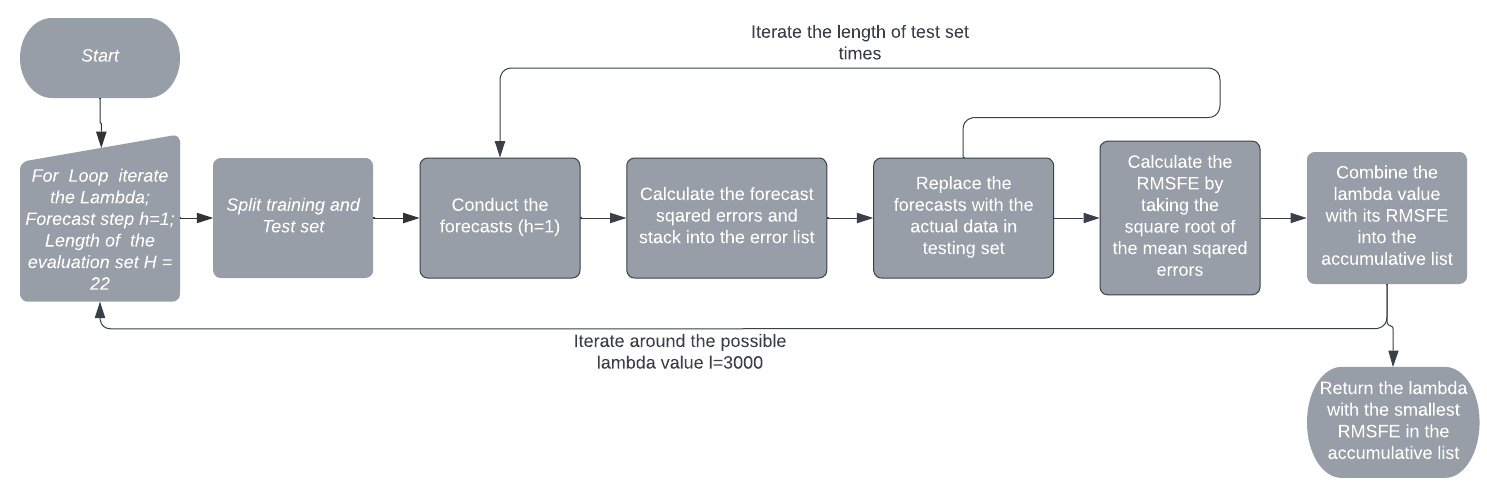
\includegraphics[scale=0.7]{Flowchart_algo}
\centering
\caption{Proposed algorithm for selecting the optimal $\lambda$}
\label{fig:sealgo}
\end{figure}

To mitigate the adverse impact of high-dimensionality, I start the algorithm from \(0.0001\), use steps of \(0.0001\) and stop at \(0.3\). There are 3000 different lambdas considered, and the algorithm will automatically return the lambda with minimum RMSFE in forecasting total number of employment (see Matlab code for this algorithm in my github file-Links in the Appendix ).

From the return value of our searching algorithm (see Figure \ref{fig:sealgo}). The estimated hyperparameter from the algorithm is \(\lambda=0.0808\), which certainly has the lowest mean scaled forecast error (RMSFE) as designed. Based on this, I choose \(\lambda=0.0808\) for subsequent analysis.

\newpage

\hypertarget{sectoral-employment-analysis}{%
\chapter{Sectoral Employment Analysis}\label{sectoral-employment-analysis}}

\hypertarget{long-run-multiplier-analysis}{%
\section{Long-run Multiplier Analysis}\label{long-run-multiplier-analysis}}

Because industries are interdependent, changes in one subsector can affect both other subsectors as well as total employment. In this chapter, the sectoral employment dynamics for each subsector will be captured using the dynamic structure of the multivariate Bayesian VAR model.

The following analysis is based on the estimated BVAR model and 84 two-digit disaggregated data. I assume that the structure of Australian economy will not change after COVID-19.

At each time point, the growth rate of total employment and the growth rates of sectoral employment satisfy the following identity:

\[
GR_T=\sum_{i=1}^{84} w_i\times {GR}_i
\]

where \(w_i\) is the share of subsector \(i\), \(GR_T\) is the growth rate of total employment and \(GR_i\) is the growth rate in employment of subsector \(i\).

In particular, if there is a one percent increase in employment in subsector \emph{i}, total employment will increase by the corresponding share(\(w_i\)) simultaneously. Additionally, given an increase in total employment, it may also have indirect effects on other sectors in consecutive periods, especially those with close economic ties. In accordance with \textcite{anderson2020}'s definition, I define the employment long-run employment multiplier as the effect of an initial increase in sector \emph{i} on total employment in the long run. If the subsector has a greater long-run effect on total employment than its immediate effect, then stimulating this sector will have a positive spillover effect on total employment.

I simulate the long-term employment multiplier for each sector over time horizons of one year, two years and ten years using the estimated Bayesian VARX model. Subsequently, the differences between the simulated ten-year multipliers and the initial shares are the spillovers of the disaggregated subsectors. I list the 10 subsectors with strongest positive spillovers alongside the 10 subsectors with strongest negative spillovers in Table \ref{fig:spl}. A comprehensive list can be found in Appendix B (see Table \ref{dis:emp}).

\begin{table}[H]
  \centering
  \caption{Disaggregated Subsectoral Long-run Employment Multipliers}
   \scalebox{0.7}{
    \begin{tabular}{|l|r|l|r|}
     \hline
    Sector/ Sub-sector &M10-M0 & Sector/ Sub-sector & M10-M0 \\
    \hline\hline
    75 Admin/ Public Administration & -0.0356327 & 42 Retail/ Other Store-Based Retailing & 0.01773361 \\
    80 Educ/ Preschool and School Education & -0.0320646 & 72 Admin/ Administrative Services & 0.01339419 \\
    81 Educ/Tertiary Education & -0.0215685 & 25Manu/ Furniture and Other Manufacturing & 0.01141447 \\
    84 Health/ Hospitals & -0.016484 & 39 Retail/ Motor Vehicle and Motor Vehicle Parts Retailing & 0.00966318 \\
    85 Health/ Medical and Other Health Care Services & -0.0112633 & 56 Info/ Broadcasting (except Internet) & 0.00736334 \\
    82 Educ/ Adult, Community and Other Education & -0.0109159 & 18 Manu/ Basic Chemical and Chemical Product Manufacturing & 0.00674883 \\
    46 Trans/ Road Transport & -0.0108955 & {33 Wholesale/ Basic Material Wholesaling} & 0.00646865 \\
    58 Info/Telecommunications Services & -0.0084901 & 13 Manu/ Textile, Leather, Clothing and Footwear Manufacturing & 0.00619223 \\
    11 Manu/ Food Product Manufacturing & -0.0082163 & 52 Trans/ Transport Support Services & 0.00617277 \\
    01 Agri/ Agriculture & -0.0076574 & 94 Other/ Repair and Maintenance & 0.00583089 \\
    \hline
    \end{tabular}}
    \begin{tablenotes} 
      \footnotesize
      \item Note: M10 is the 10-year long-run total employment multiplier and M0 is the shares of each sector.
      ;The M10-M0 is the spillover effect.;
      The M10/M0 is the spillover effect relative to the size of sector.
    \end{tablenotes}
  \label{fig:spl} 
\end{table}

Comparing the long-term multipliers with the shares, we discover that ``Other Store-Based Retailing'' \footnote{This subsector contains the following groups: 421. Furniture, Floor Coverings, Houseware and Textile Goods Retailing; 422. Electrical and Electronic Goods Retailing; 423. Hardware, Building and Garden Supplies Retailing; 424. Recreational Goods Retailing; 425. Clothing, Footwear and Personal Accessory Retailing; 426. Department Stores; 427. Pharmaceutical and Other Store-Based Retailing} will generate the greatest positive spillover effects on total employment, followed by ``Administrative Services''\footnote{This subsector contains the following groups: 721. Employment Services; 722. Travel Agency and Tour Arrangement Services; 729. Other Administrative Services.}, and ``Furniture and Other Manufacturing''. At the broadest level, these subsectors fall under the ``Retailing'', ``Administrative and Support Services'' and ``Manufacturing'' sectors respectively. These results suggest that total employment will increase over and above the initial increase in these sectors if there is an exogenous increase in these sectors.

There are also some interesting points to be noticed here. First, both the sign and the magnitude of spillover effect are not solely dependent the size of subsectors. For instance, ``Fishing, Hunting and Trapping'' is the smallest sector (see Table \ref{dis:emp}). Nevertheless, it generates positive spillovers. In addition, ``Furniture and Other Manufacturing'' is a relative small subsector but generate stronger spillover than ``Food and Beverage Services'', a relative large subsector\footnote{The share of ``Furniture and Other Manufacturing'' is 0.00496526, whereas the share of ``Food and Beverage Services'' is 0.06348661}. Contrarily, both the ``Professional, Scientific and Technical Services'' and ``Construction Services'', which are large subsectors but generate negative spillovers in the long run.

Second, I discover that subsectors in the ``Construction'' sector\footnote{Construction Sector contains three subsectors: 30. Building Construction; 31. Heavy and Civil Engineering Construction;32. Construction Services} may not bring strong positive spillovers in the two-digit level, which is in contrast to the result concluded by \textcite{anderson2020}. The ``Construction Service'' subsector, for example, will not have positive spillovers even though the overall spillover effect of the ``Construction'' sector being positive\footnote{The spillover for the ``Construction'' sector is equal to the sum of all its subsectors (-0.0004619 + 0.00271218 +0.00066987 = 0.00292015). In this case, it is still positive but no longer strong.}. This further demonstrates the necessity of expanding the research to a finer partition (more disaggregated level)

Third, both ``Tertiary Education'' and ``Adult, Community and Other Education'' generate negative spillovers, which implies that stimulating the education industry will probably reduce total employment in the long run. This is mainly because if one decides to pursue a postgraduate degree or a certificate, then the focus will shift away from working/finding jobs. The results are also in line with the broadest level (19 sectors) analysis that undertaken by \textcite{anderson2020}.

\hypertarget{evaluations-after-covid-19}{%
\section{Evaluations after COVID-19}\label{evaluations-after-covid-19}}

\hypertarget{losses-of-total-employment}{%
\subsection{Losses of Total Employment}\label{losses-of-total-employment}}

Based on the fact that COVID-19 can spread quickly and there is no wonder drug to prevent outbreaks of new variants so far, we will never be able to completely halt the virus' spread or prevent infection unless there is no human contact. As a result, it is anticipated that COVID-19 has caused massive losses to the Australian labour market and these negative effects will be persistent in the long run. To prove my idea and raise awareness about COVID-19, I will conduct a counterfactual analysis by evaluating the difference of total employment with and without the pandemic. In this section, I use the estimated model to conduct a counterfactual analysis for total employment after the pandemic. Similar to \textcite{anderson2020}, I will consider a ``no-COVID'' scenario. In light of the fact that the pandemic has already occurred, other scenarios are not taken into account. Recent data will be used to compare and evaluate the effects of COVID-19 on the labour market.

\begin{figure}[H]
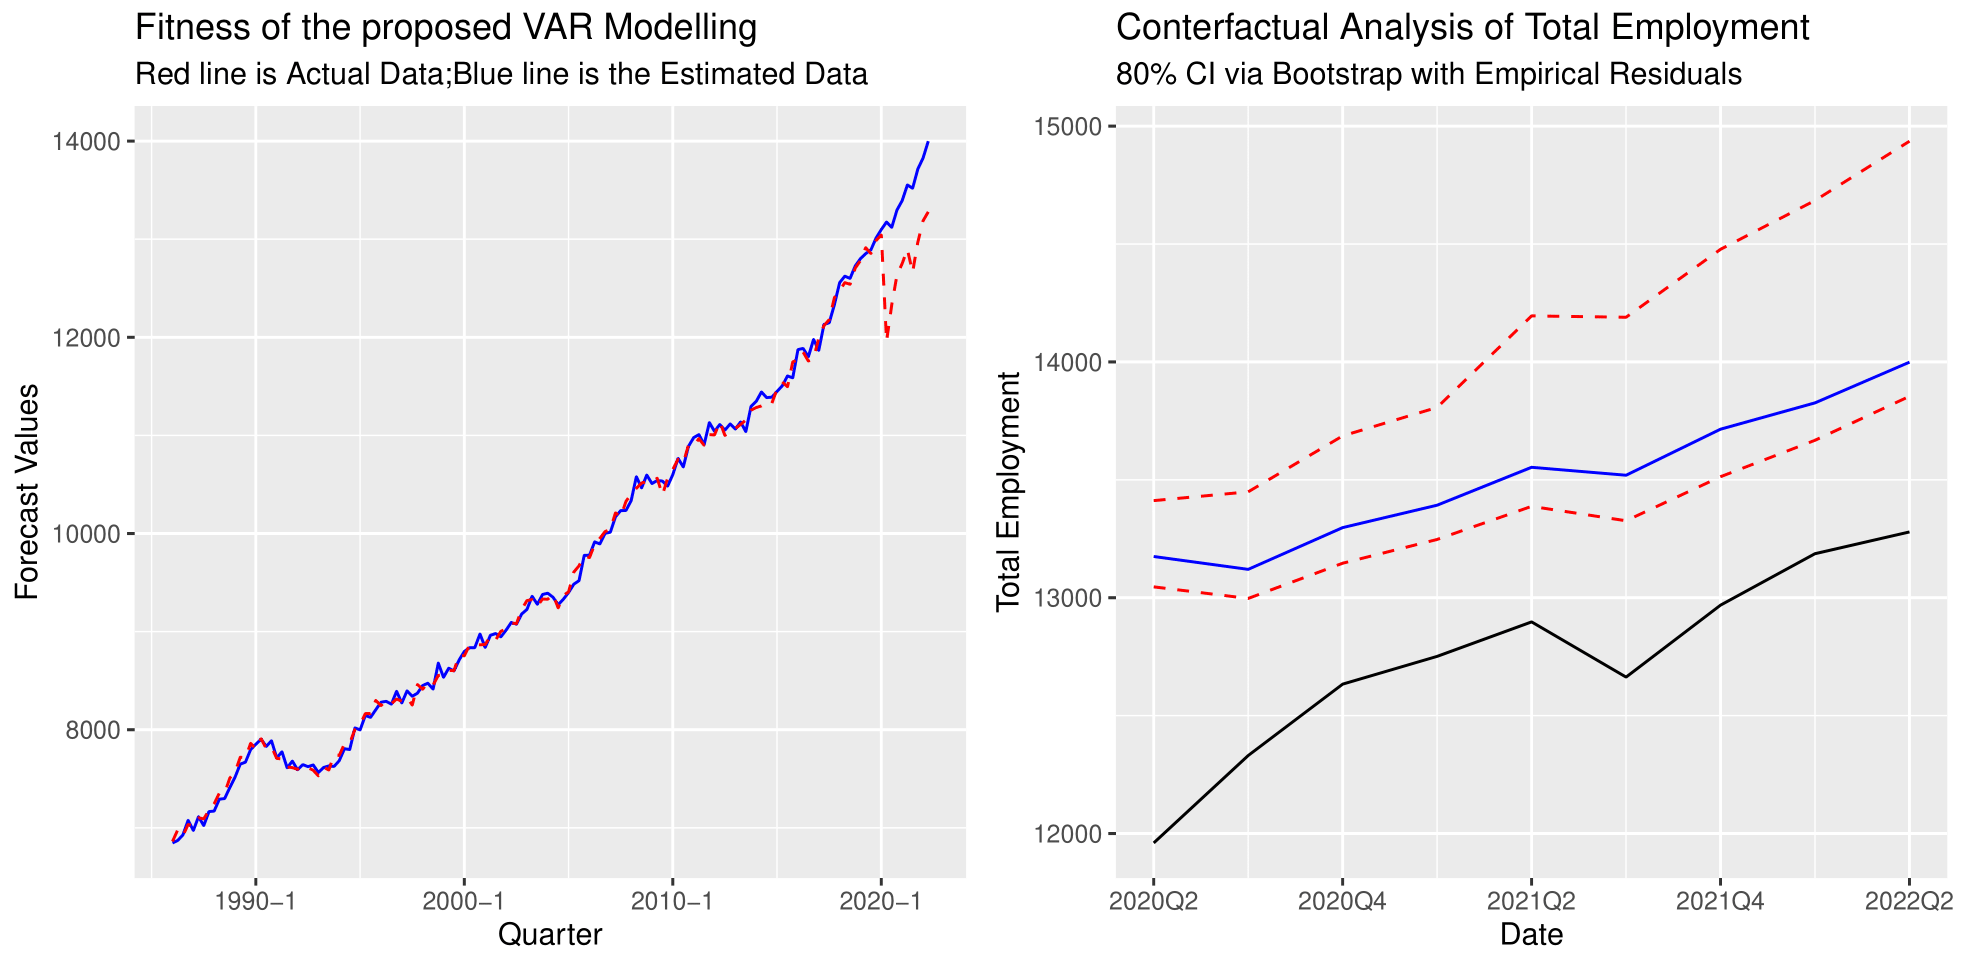
\includegraphics[scale=0.6]{cont_analysis}
\centering
\caption{Counterfactual analysis of total employment(in thousands) with confidence interval generated via bootstrap (Blue is counterfactual scenario (no-COVID);Black is the actual data)}
\label{fig:con}
\end{figure}

Figure \ref{fig:con} displays COVID-19 has caused a continuous structural shock of total employment in Australia since the outbreak of COVID-19. Based on the point forecasts together with an 80\% confidence interval (via empirical bootstrap\footnote{As there are 7224 parameters to estimate, we do not use the Bayesian prediction intervals concerning the time complexity required when taking high-dimensional integrals.}), our model indicates that employment losses remained at approximately 750,000 persons below where it would have been without the pandemic (see the differences in Figure \ref{fig:con}). By comparing the trend of the ``no-pandemic'' scenario and that of the actual data, the essentially parallel trend revealed that we may not expect total employment to attain the forecasts under the no-COVID case in the anticipated future. That is, COVID-19 has had a long-lasting effect on the economy even after two years of the primary lockdown in 2020 ``Quarter 2''.

\begin{figure}[H]
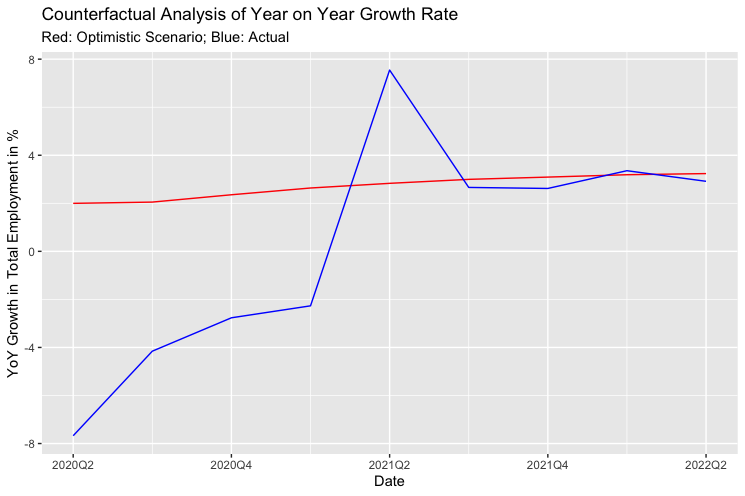
\includegraphics[scale=0.6]{yoy1}
\centering
\caption{Counterfactual analysis of Year-on-Year growth rate (forecasts generated via the estimated BVAR model)}
\label{fig:yoy}
\end{figure}

Additionally, I have also considered the Year-on-Year growth rate for quarterly total employment data from 2020 Q2 to 2022 Q2 (up-to-date at the time of collecting). According to Figure \ref{fig:yoy}, the actual employment growth was far below from the expected growth, particularly in 2020 Q2, when Australia was experiencing the first lockdown. After that, the year-on-year growth rate gradually recovered back to ``no-COVID'' forecasts,but total employment is still lower than it would be under the ``no-COVID'' situation. Again, it has been emphasized the finding above and we may not expect the influences of COVID-19 to disappear unless there is a higher year-on-year growth rate and persists for a while in the future. Therefore, it is reasonable to assume that COVID-19 has indeed a significant impact on the labour market both in the short term as well as in the long term based on the counterfactual analysis of employment and the year-on-year growth rate.

\hypertarget{an-explanation-for-the-historically-low-unemployment-rate}{%
\subsection{An explanation for the historically low unemployment rate}\label{an-explanation-for-the-historically-low-unemployment-rate}}

In June 2022, Australia fell to its the lowest unemployment rate since August 1974 (\textcite{ABS2022a}). Then one might be interested in learning what the underlying reason for this incredibly low unemployment rate. Are the stimulus policies during COVID-19 that have contributed the most to the low unemployment rate? In answering this question, I will use a counterfactual analysis of the unemployment rate to exploit why and what the unemployment rate would have been without the pandemic case.

To give an accurate interpretation of the low unemployment rate, the answer should refer to the definition, which is the percentage of people who are in the labour force but are unemployed. Mathematically, it is:

\[
\begin{aligned}
\text{Unemployment Rate}=\frac{Total\ Labour\  Force- Number\ of \ Employed \ People}{Total\ Labour \ Force}
\label{equ:unemp}
\end{aligned}
\]

It is obvious that the unemployment rate depends on both the total labour force and the number of employed people. According to the estimated BVAR model suggests that employment is less than it would have been in the absence of COVID (see \emph{Chapter 5}). Therefore, given the low unemployment rate and fewer employed people than in the no-COVID scenario, one explanation might be a significant drop in the total labour force after the pandemic.

To further support this hypothesis, I use quarterly labour force data from ABS from ``1984 Q4'' to ``2022 Q2'' \autocite{ABS2022}. In addition, a stepwise \texttt{ARIMA} model \autocite{fpp3} is used to fit the ``no-COVID'' data between ``1984 Q4'' and ``2020 Q1'' to forecast the total labour force under the ``no-COVID'' scenario (see Figure \ref{fig:lab}). Compared with the actual data, it is evident that the real total labour force is lower than the ``no-COVID'' forecasts at the time when the unemployment rate is at its lowest historically. Therefore, rather than the effects of stimulus policies during the pandemic period, the main reason for the low unemployment rate is the decline in the total labour force.

\begin{figure}[H]
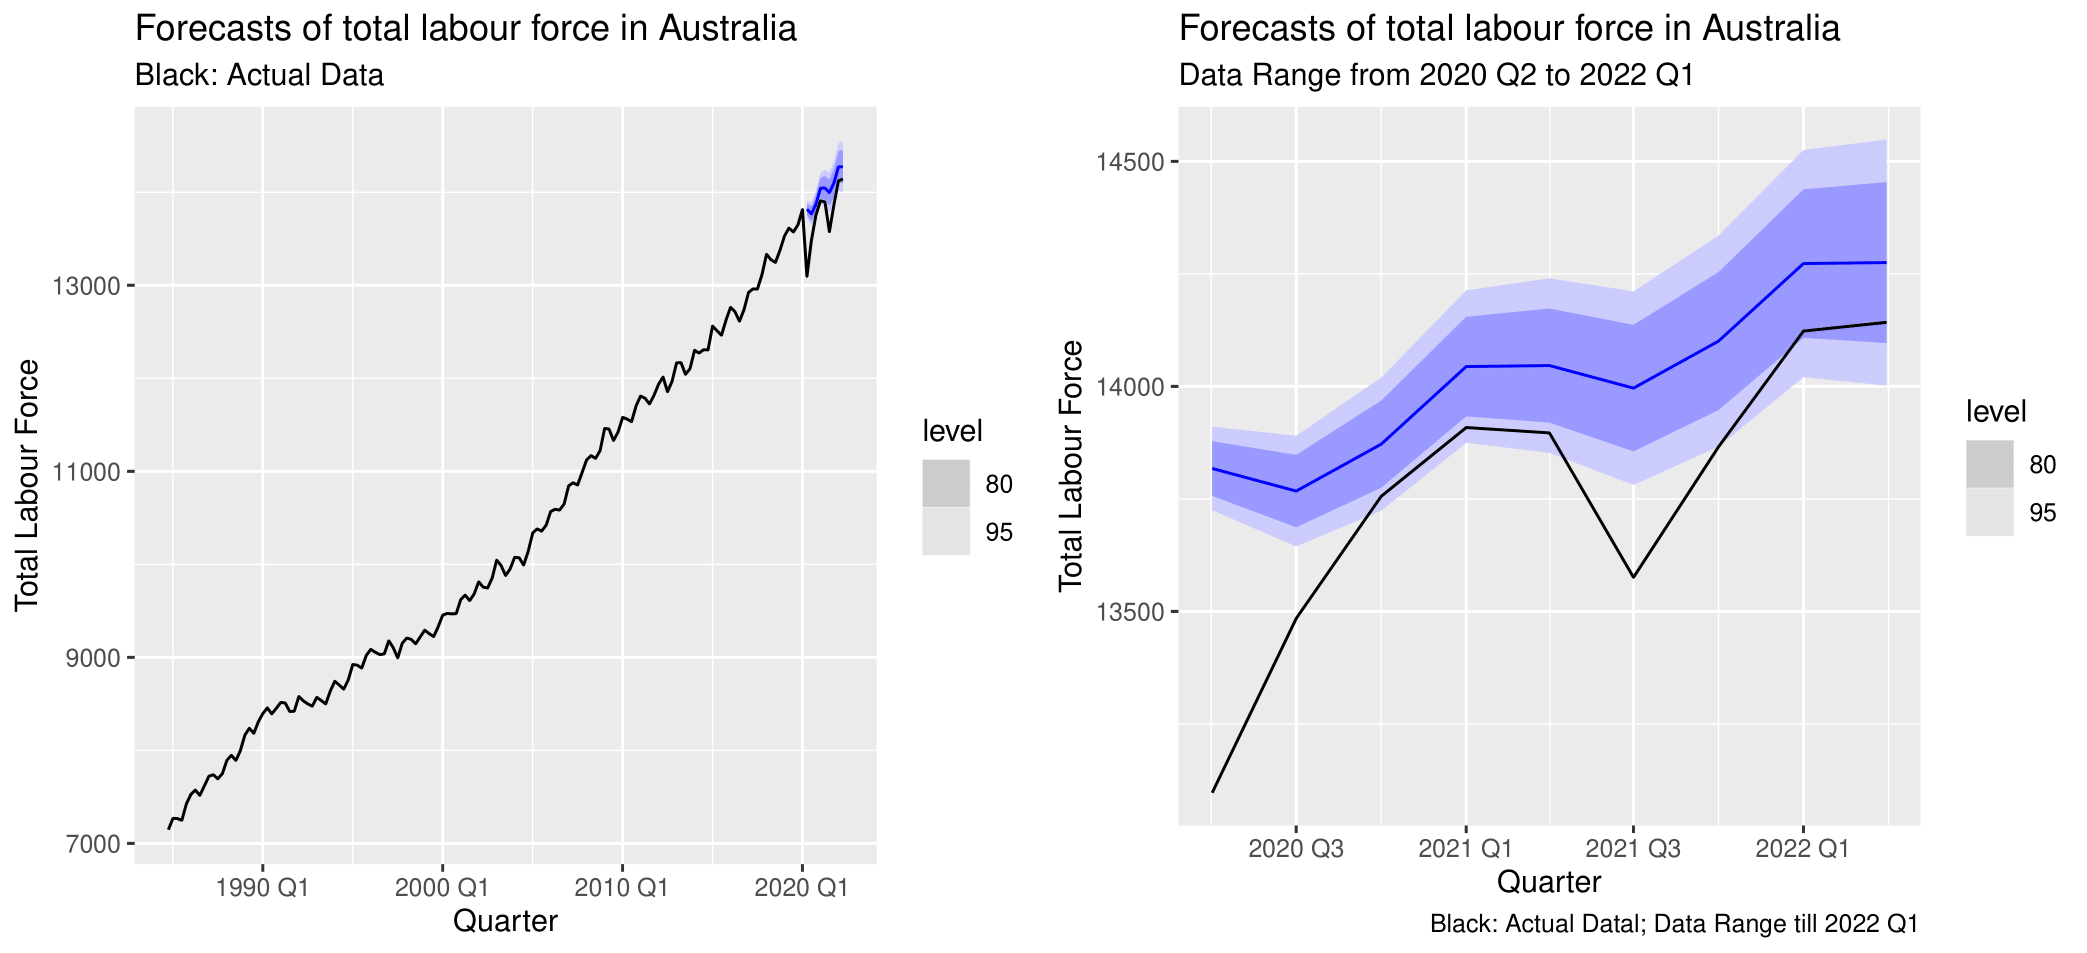
\includegraphics[scale=0.6]{con_labourf}
\centering
\caption{Counterfactual analysis of the total labour force (Blue: the forecasts under the no-COVID scenario, Black is the Actual Data)}
\label{fig:lab}
\end{figure}

After looking into the underlying reason for the low unemployment rate, I also studied how the unemployment rate would perform in the absence of COVID-19. The forecasts of the no-COVID unemployment rate is calculated as the difference between the total labour force and employment rate over the total labour force under the no-COVID scenario. It is noteworthy that the anticipated unemployment rate (under no-COVID scenario) can still be the lowest on record, even with a larger labour force and total employment.

Overall, the findings suggest that we would have experienced the historically low unemployment rate even in the absence of COVID-19. This further assures us that the policies directed at stimulating employment during the pandemic (e.g.~Jobkeeper program) are unlikely to be responsible for the current historically low unemployment rate.

\begin{figure}[H]
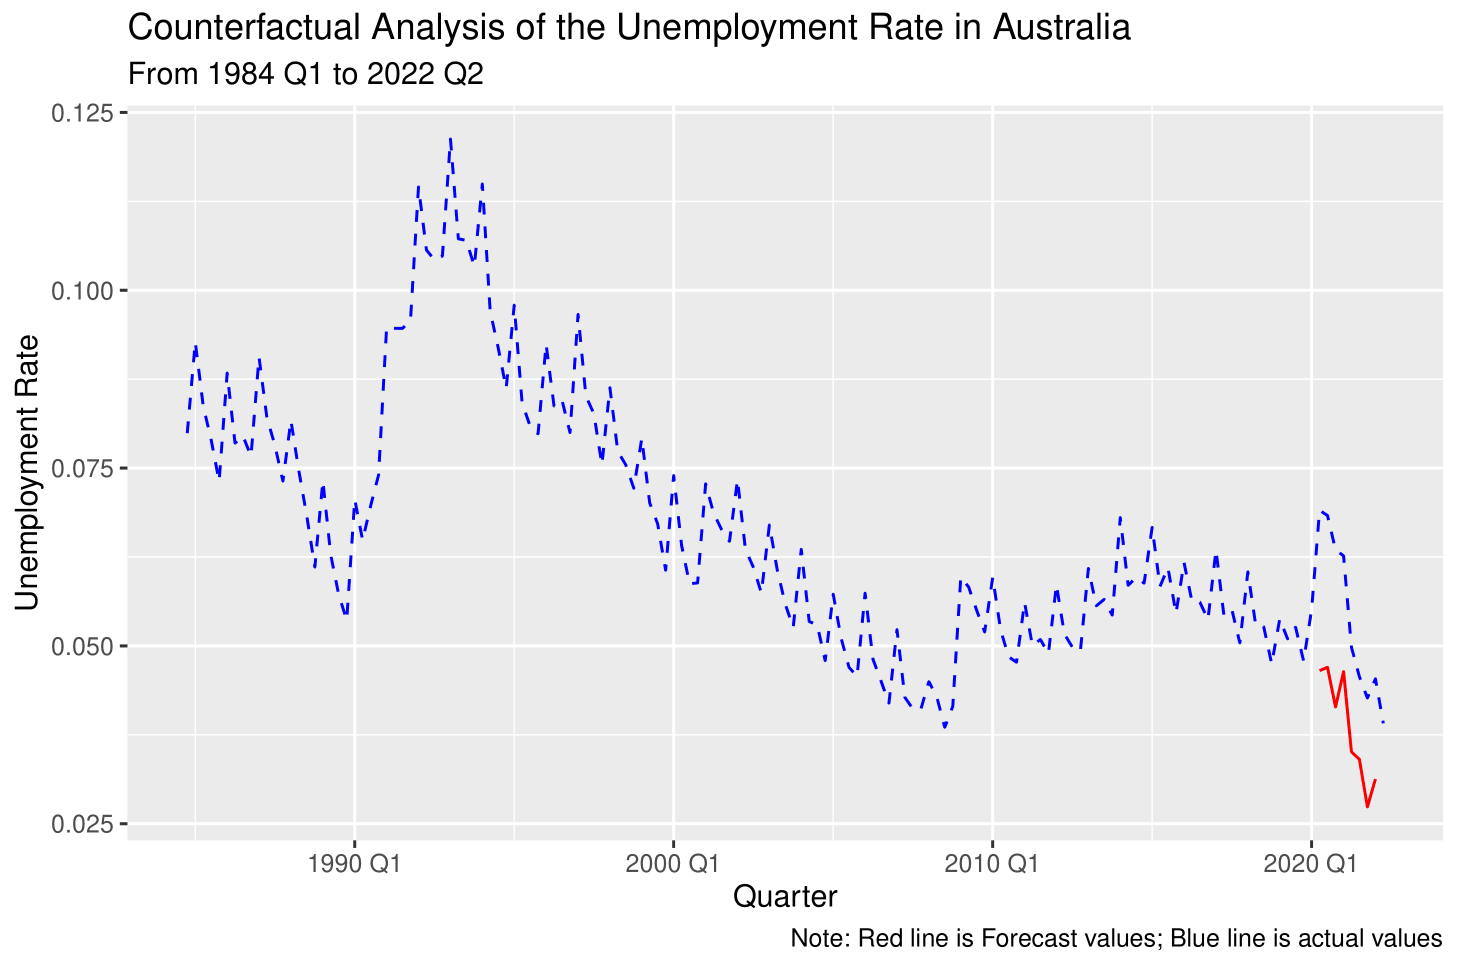
\includegraphics[scale=0.7]{unempcont}
\centering
\caption{Counterfactual analysis of the unemployment rate in Australia}
\label{fig:unrate}
\end{figure}

\clearpage

\hypertarget{discussions-and-conclusion}{%
\chapter{Discussions and conclusion}\label{discussions-and-conclusion}}

In conclusion, I have developed a dynamic Bayesian VAR (BVAR) system to analyse the two-digit employment dynamics in Australia. This allows me to view the Australian employment market from a new perspective. First, an out-of-sample forecasting algorithm was proposed to select the most optimal hyperparameter in Minnesota Prior and also to improve the forecast accuracy. Second, I conducted the spillover analysis using the estimated model to discover how total employment reacts in the long run when the subsectors are stimulated. Based on the result, ``Other Store-Based Retailing'', followed by ``Administrative Services'', ``Furniture and Other Manufacturing'' will generate strong positive spillovers in employment. In particular, they will maker greater contributions to total employment than their original sizes (i.e.~the shares of subsectors). It is helpful for policymakers to consider industries that could operate efficiently, and act as the backbone of the economy (i.e.~high-spillover industries) when formulating policies to stimulate the economy.

Furthermore, I evaluate the shocks of COVID-19 to the Australian labour market with the estimated BVAR model. This counterfactual analysis end up with a conclusion that these structural shocks in fact have a long-term negative impact. As a result, it will be challenging to completely mitigate the influences of the pandemic in the foreseeable future. To shed light on the reason for the low unemployment rate in Australia, I conduct an empirical analysis and compare the estimated unemployment rate in the absence of the pandemic with actual values. Results suggest that labour force is less than it would have been without the pandemic, and we would have experienced a low unemployment rate even in the absence of COVID-19. Given these points, I identify that the low unemployment rate is mainly driven by the loss of the total labour force rather than the stimulus policies during the pandemic.

\hypertarget{limitation}{%
\section{Limitation}\label{limitation}}

There are few non-classified data (nfd data) under each sector in the ABS employment by subdivision dataset \autocite{ABS2022}. Data that are not classified have not been considered in this study. This is mainly because the data is not evenly distributed, which will be problematic if we simply distribute it into our system by the share of each subsector.I haven't yet thought of a good way to distribute the data. In the future, it would be great to come up with some effective ways (e.g.~Contact ABS about detailed information) to trace the source of them. Consequently, the total employment data used in this thesis is not the same as the published total employment data as we discussed in \emph{Chapter 3.1}. Nevertheless, we only consider the ANZSIC subdivision in our case (two-digit sectors). In the future, it would be beneficial to consider using both the Division level (the broadest level) and the group and classes (the finest level) using hierarchical forecasting. The predictions we examined are based on the assumption that the parameter of the model has been constant thought the time before COVID-19 and structure will not change after COVID-19, which might be restrictive. An appropriate time-varying model could be implemented to have more flexibility in modelling dynamics.

\hypertarget{future-extension-an-application-of-machine-learning-in-hierarchical-forecasting}{%
\section{Future Extension: An Application of Machine Learning in Hierarchical Forecasting}\label{future-extension-an-application-of-machine-learning-in-hierarchical-forecasting}}

In this research, the Bayesian VAR modelling method has provided a useful analysis of employment dynamics in Australia. However, VAR modelling may be inefficient, when there is more data and hierarchies are considered. Therefore, a more efficient machine learning technique could be considered as an extension of the hierarchical forecasting.

To improve the forecast accuracy, we could use machine learning to give a new way that accounts for both accuracy and interpretability. First, pick up the common features or data types from the data and cluster them into groups based on them. Second, conduct group-based forecasting for each new cluster. Then, we can reconcile them to be coherent, which will benefit the decision and policy implementation processes.

Here, I will give an example of the machine learning algorithm.

\begin{enumerate}
\def\labelenumi{\arabic{enumi}.}
\item
  Cluster-bottom level data based on common features (e.g.~domain-specific features, time series characteristics etc.) via possible machine learning algorithms (e.g.~manifold learning, k-means).
\item
  Create a model to forecast each time series within the same cluster. Although it seems restrictive, there are two points should be helpful in proving both accuracyc and flexibility. First, the choice of model is flexible andcan be complex. There are many types of models to choose from, depending on the domaintypes and time series patterns. Moreover, the types of models are not limited, which canbe either a single model (e.g.~univariate, multivariate, and ML) or a combined model(e.g.~Weighted average of various forecasting methods). Second, forecasting methods canbe different for different clusters of the data, due to some unique patterns in time series.
\item
  Reconcile the forecasts produced by the machine learning algorithm to make them coherent. To get more interpretable results, reconciliation is required to fit all forecasts produced in our clusters into the original structure of the data (i.e.~the original groups).
\end{enumerate}

\appendix

\hypertarget{an-example-of-bayesian-var-and-minnesota-prior}{%
\chapter{An Example of Bayesian VAR and Minnesota Prior}\label{an-example-of-bayesian-var-and-minnesota-prior}}

The VARX model is:

\[
\begin{aligned}
\bm{y}_t&=\bm{c}+\bm{A}_1 \bm{y}_{t-1}+\bm{\Gamma}_1\bm{x}_{t-1}+\bm{u}_t\\
&=
\begin{bmatrix}
c_1\\
\vdots\\
c_n
\end{bmatrix}
+
\begin{bmatrix}
a_1^{11}&\cdots&a_1^{1n}&\gamma_1^{1}\\
\vdots&\ddots&\vdots&\vdots\\
a_1^{n1}&\cdots&a_1^{nn}&\gamma_1^n\\
\end{bmatrix}
\begin{bmatrix}
\bm{y}_{t-1}\\
x_{t-1}\\
\end{bmatrix}\\
&+
\begin{bmatrix}
u_{1,t}\\
\vdots\\
u_{n,t}
\end{bmatrix}\\
\end{aligned}
\]

where \(\bm{y_t} = ln(\bm{z_t})-ln(\bm{z_{t-4}})\) and \(z_t\) is the number of employment in subsectors; \(\mathbb{E}(\bm{u}_t\bm{u}'_t)=\bm{\Sigma}\) and \(\mathbb{E}(\bm{u}_t\bm{u'}_{t-1})=0\). Here the \(n\) represent the number of sectors (in our case this will be 84) and \(\bm{c}\)represents the vector of constants. There is one lag (p=1) included of the total employment growth for each equation \((x_{t-1})\) as a predetermined variable at time \(t\).

We estimate the VARX using Bayesian method via a natural-conjugate-Normal-Wishart prior which preserve the properties of the Minnesota prior. We apply the shrinkage to the VAR slope coefficients using a Minnesota Prior specification as follows:

\[
\begin{aligned}
&E[a_{i}^{jk}] = E[\gamma_{i}^j]=0\\
\\
&Var[a_i^{jk}]= 
\begin{cases}
\frac{\lambda^2}{i^2},&j=k\\
\frac{\lambda^2}{i^2}\frac{\sigma^2_{j}}{\sigma^2_k},& otherwise
\end{cases}\\
\\
&Var[\gamma_i^{j}]=\frac{\lambda^2}{i^2}\frac{\sigma^2_{j}}{\sigma^2_e}
\end{aligned}
\]

The \(\sigma^2_{t}\) is estimated by taking the residual variances after fitting an AR(4) on the \(l^{th}\) variable using least squares, which is common practice (see \textcite{anderson2020};\textcite{banbura2010large}). The degree of shrinkage is governed by \(\lambda\) and the \(i\) stands for number of lags. \(\frac{\sigma^2_{j}}{\sigma^2_e}\) adjust different scales of the data. The \(\lambda\) we apply in this thesis is selected in \emph{Chapter 4.3}.

The nature conjugate Normal-Inverse-Wishart prior implies the posterior moments can be calculated either analytically or by using the dummy observations.

Then we implement our VAR by defining \((np+n+1)\) dummy observations:

To estimate the BVAR using dummy observations, we rewrite the estimated model as
\[
\begin{aligned}
\bm{Y} = \bm{X}\bm{\beta}+\bm{u}
\end{aligned}
\]
where we set the prior parameters as \(\bm{Y} = [\bm{y_1},\cdots,\bm{y_t}]\), \(\bm{X} = [\bm{X_1},\cdots,\bm{X_T}]\) where \(\bm{X_t}=[\bm{y_{t-1}}, x_{t-1}]\) and \(\bm{u} = [u_1,\cdots,u_T]\).

The Normal-Wishart prior distribution then take the form:

\[
\begin{aligned}
vec(\bm{\beta})|\bm{\Sigma} \sim \bm{N}(vec(\bm{\beta_0}),\bm{\Sigma}\otimes \bm{\Omega_0})), and\\
\Sigma \sim IW(\bm{S_0},a_0)
\end{aligned}
\]
where we set the prior parameters \(\bm{\beta_0}\), \(\bm{\Omega_0}\), \(\bm{S_0}\) and \(a_0\) such that they are consistent with the Minnesota Prior setting.

The expectation of \(\bm{\Sigma}\) being \(diag(\sigma^2_{1},\cdots,\sigma^2_{n})\). We follow \textcite{anderson2020} to set our prior by defining dummy observations:

\[
\begin{aligned}
\bm{Y_d}&=
\begin{pmatrix}
\bm0_{np+p,n}\\
diag({\sigma_1,\cdots,\sigma_n})\\
\bm0_{1\times n}
\end{pmatrix},\\
\bm{X_d}&=
\begin{pmatrix}
\bm{J_p}\otimes diag(\frac{\sigma_1}{\lambda}\cdots\frac{\sigma_n}{\lambda},\frac{\sigma_e}{\lambda})&\bm0_{(np+p)\times1}\\
\bm 0_{n,np+p}&\bm 0_{n\times1}
\\
\bm 0_{1,np+p}&\bm{\epsilon}
\end{pmatrix},
\end{aligned}
\]

where \(\bm{Y_d}\) and \(\bm{X_d}\) are the dummy observations chosen according to the Minnesota Prior assumption (consistent with the mean and variance setups above).

\[
\begin{aligned}
\bm{J_p}=diag(1,\cdots,p),\\
\bm{S_0}=(\bm{Y_d}-\bm{X_d} \bm{B_0})'(\bm{Y_d}-\bm{X_d}\bm{B_0}),\\
\bm{B_0}=(\bm{X_d}'\bm{X_d})^{-1}\bm{X_d}\bm{Y_d},\ \bm{\Omega_0}=(\bm{X_d}'\bm{X_d})^{-1}\  and\\
a_0=T_d-np-p-1, \\
\end{aligned}
\]

where \(T_d\) is the number of rows for both \(\boldsymbol{Y}_d\) and \(\boldsymbol{X}_d\). \(\epsilon\) is a very small number to impose an uninformative and diffused prior on the constants. The first block of the dummy observations imposes the prior belief on the VAR slope coefficients and the second block contains the prior for the covariance matrix and third block imposes the prior belief on the constants.

Then we augment the original BVAR model with the estimated dummy observations. We can get:

\[
\begin{aligned}
\bm{Y^*}=\bm{X^*}\bm{\beta}+\bm{\mu}^*\ \ \  where: \\
\bm{Y^*}=[\bm{Y'},\bm{Y'_d}]';\ \bm{X^*}=[\bm{X'},\bm{X'_d}]';\ \bm{\mu^*}=[\bm{\mu'},\bm{\mu'_d}]'
\end{aligned}
\]

Then we can estimating the BVAR by conducting least squares regression of \(\boldsymbol{Y}^*\) on \(\boldsymbol{X}^*\). The posterior distribution then has the form of

\[
\begin{aligned}
&vec(\bm{\beta})|\bm{\Sigma},\bm{Y}\sim N(vec(\boldsymbol{\tilde\beta}),\boldsymbol{\Sigma}\otimes(\boldsymbol{X^*}'\boldsymbol{X^*})^{-1})\ and\\
&\bm{\Sigma}|\bm{Y}\sim\bm{IW}(\bm{\tilde\Sigma},T_d+T-np+2)
\end{aligned}
\]

where \(\bm{\tilde\beta} =({\bm{X^{*}}}'\bm{X^{*}})^{-1} {\bm{X^{*}}}'\bm{Y^{*}}\) and \(\bm{\tilde\Sigma}=(\bm{Y^{*}}-\bm{X^{*}}\bm{\tilde\beta})'(\bm{Y^{*}}-\bm{X^{*}}\bm{\tilde\beta})\)

\hypertarget{graphs}{%
\chapter{Graphs}\label{graphs}}

\graphicspath{ {/Users/elvisyang/Desktop/hon_proj/Disaggregated_Employment/Honours_thesis/figures} }

\begin{figure}[t]
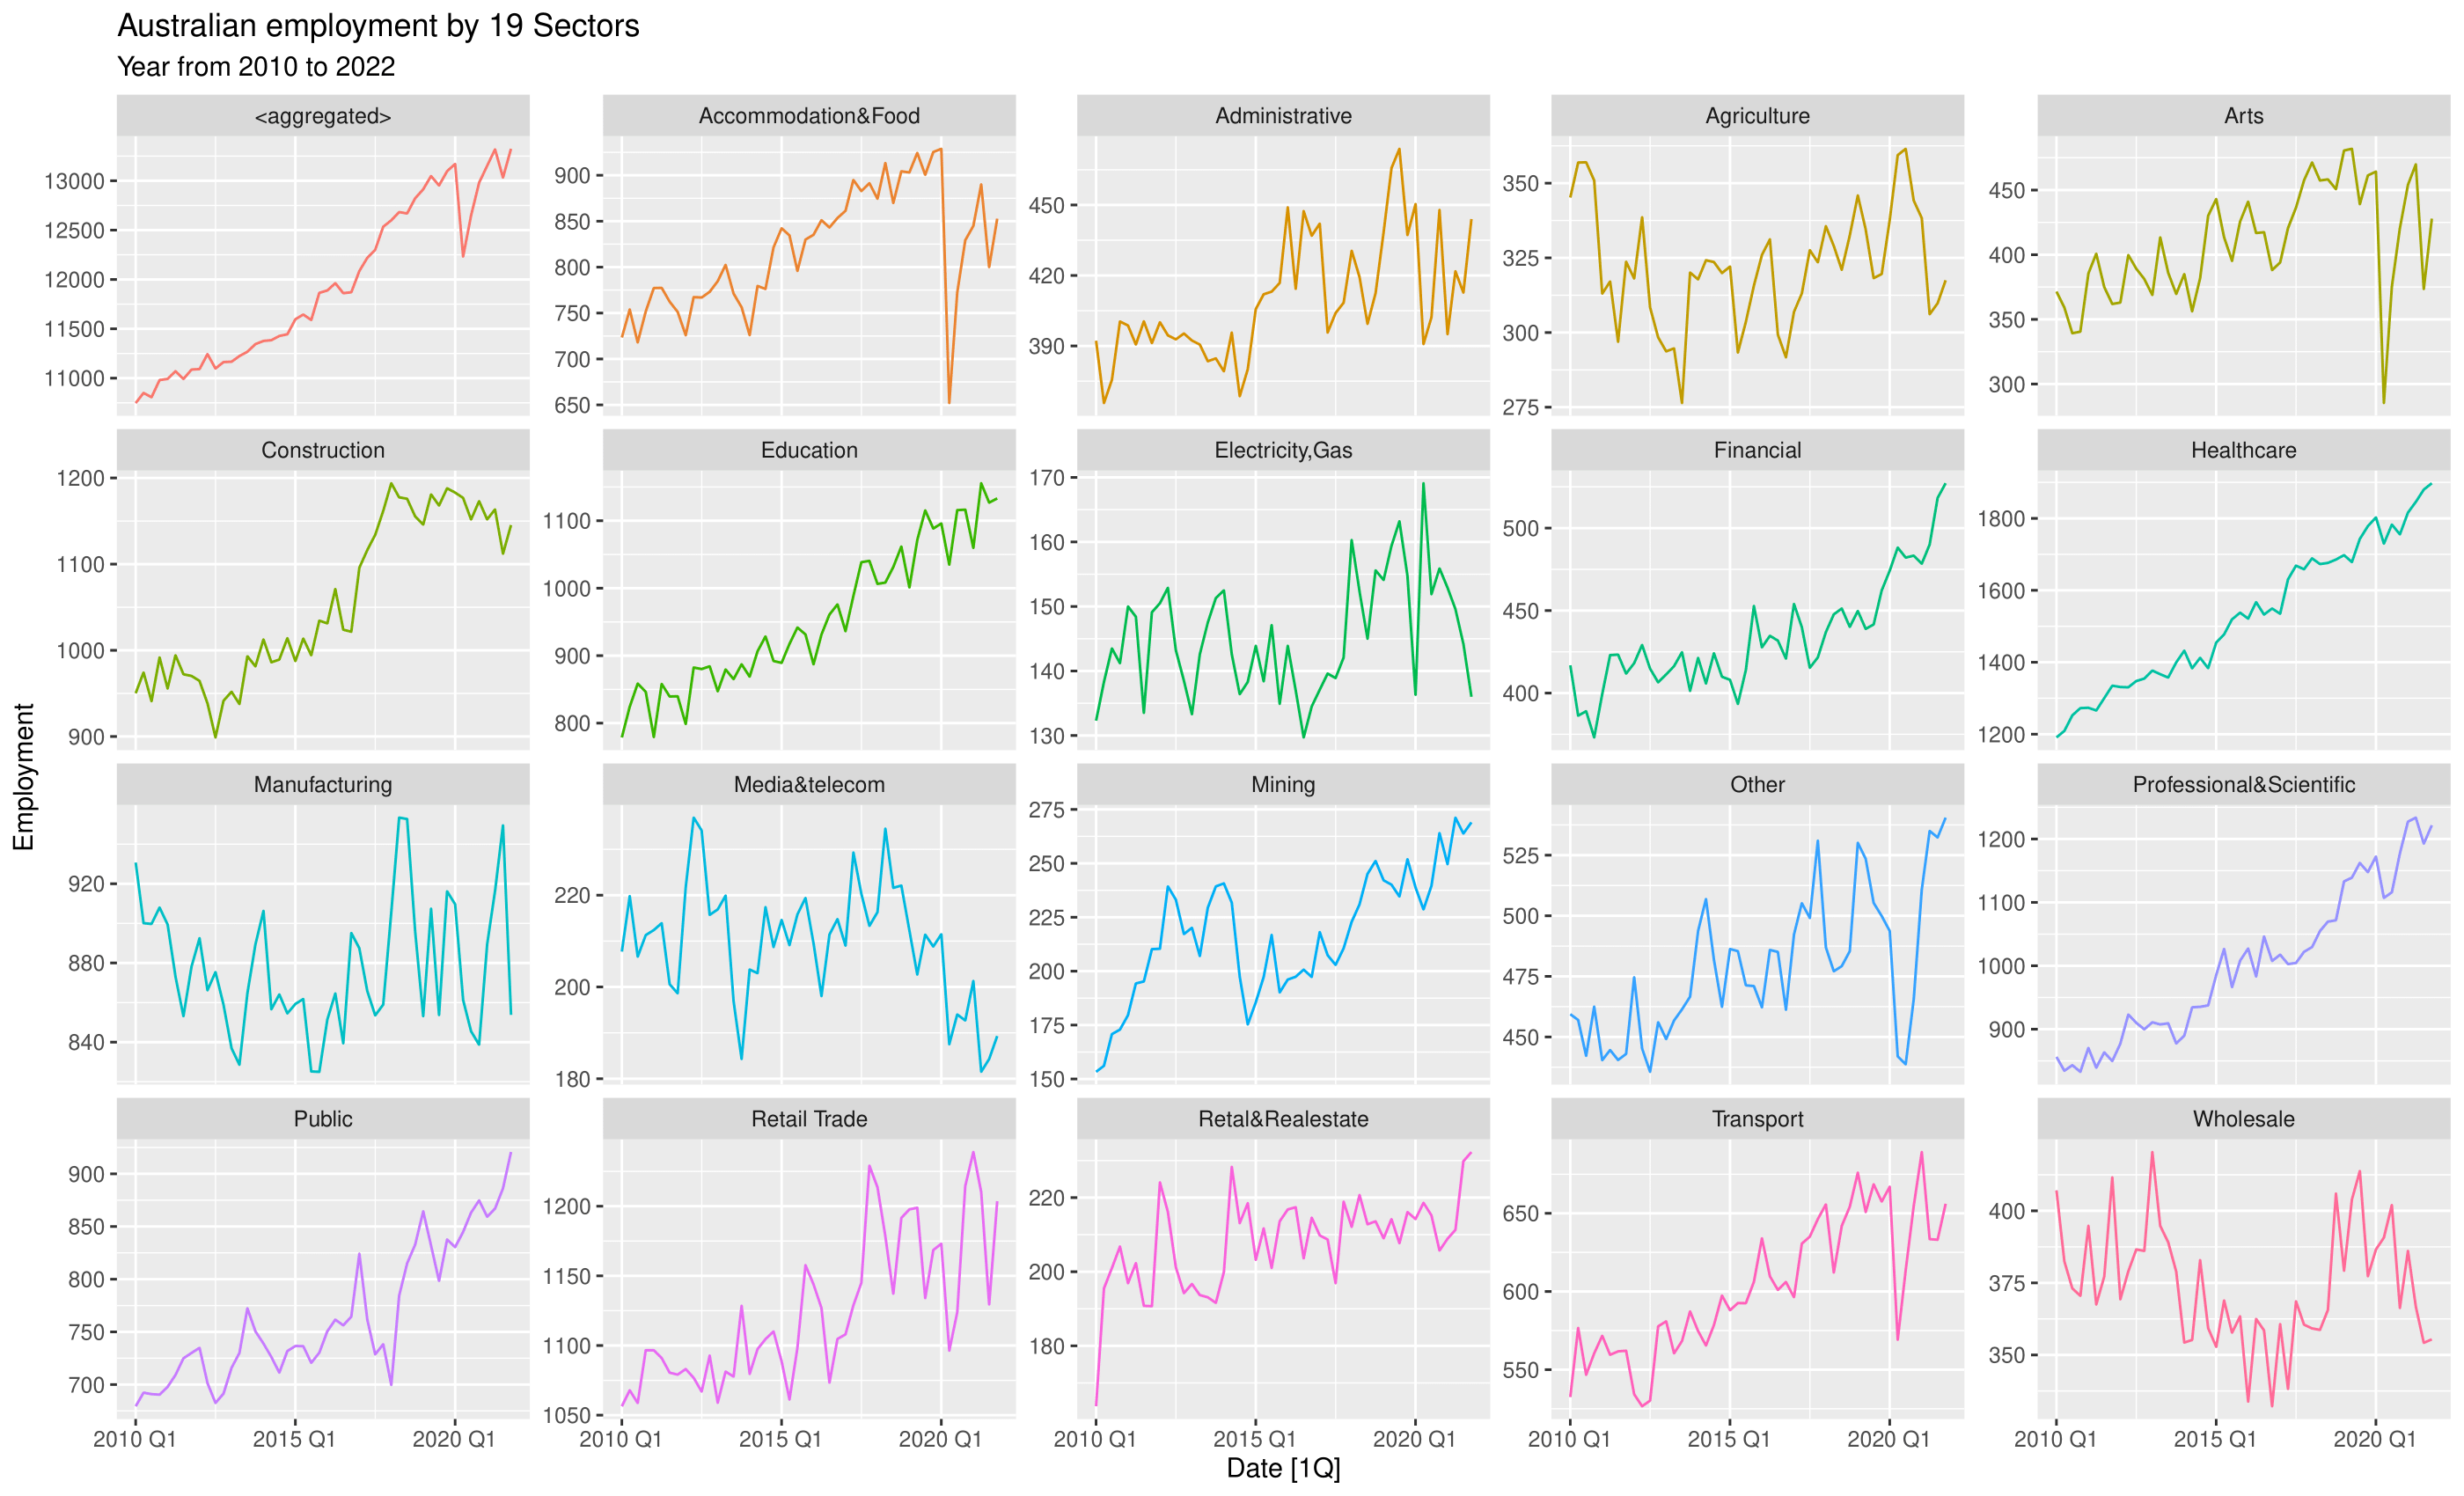
\includegraphics[scale=0.5]{19sec}
\centering
\caption{Employment('000) of 19 sectors in Australia from 2010 to 2022}
\label{fig:19}
\end{figure}

\begin{figure}[t]
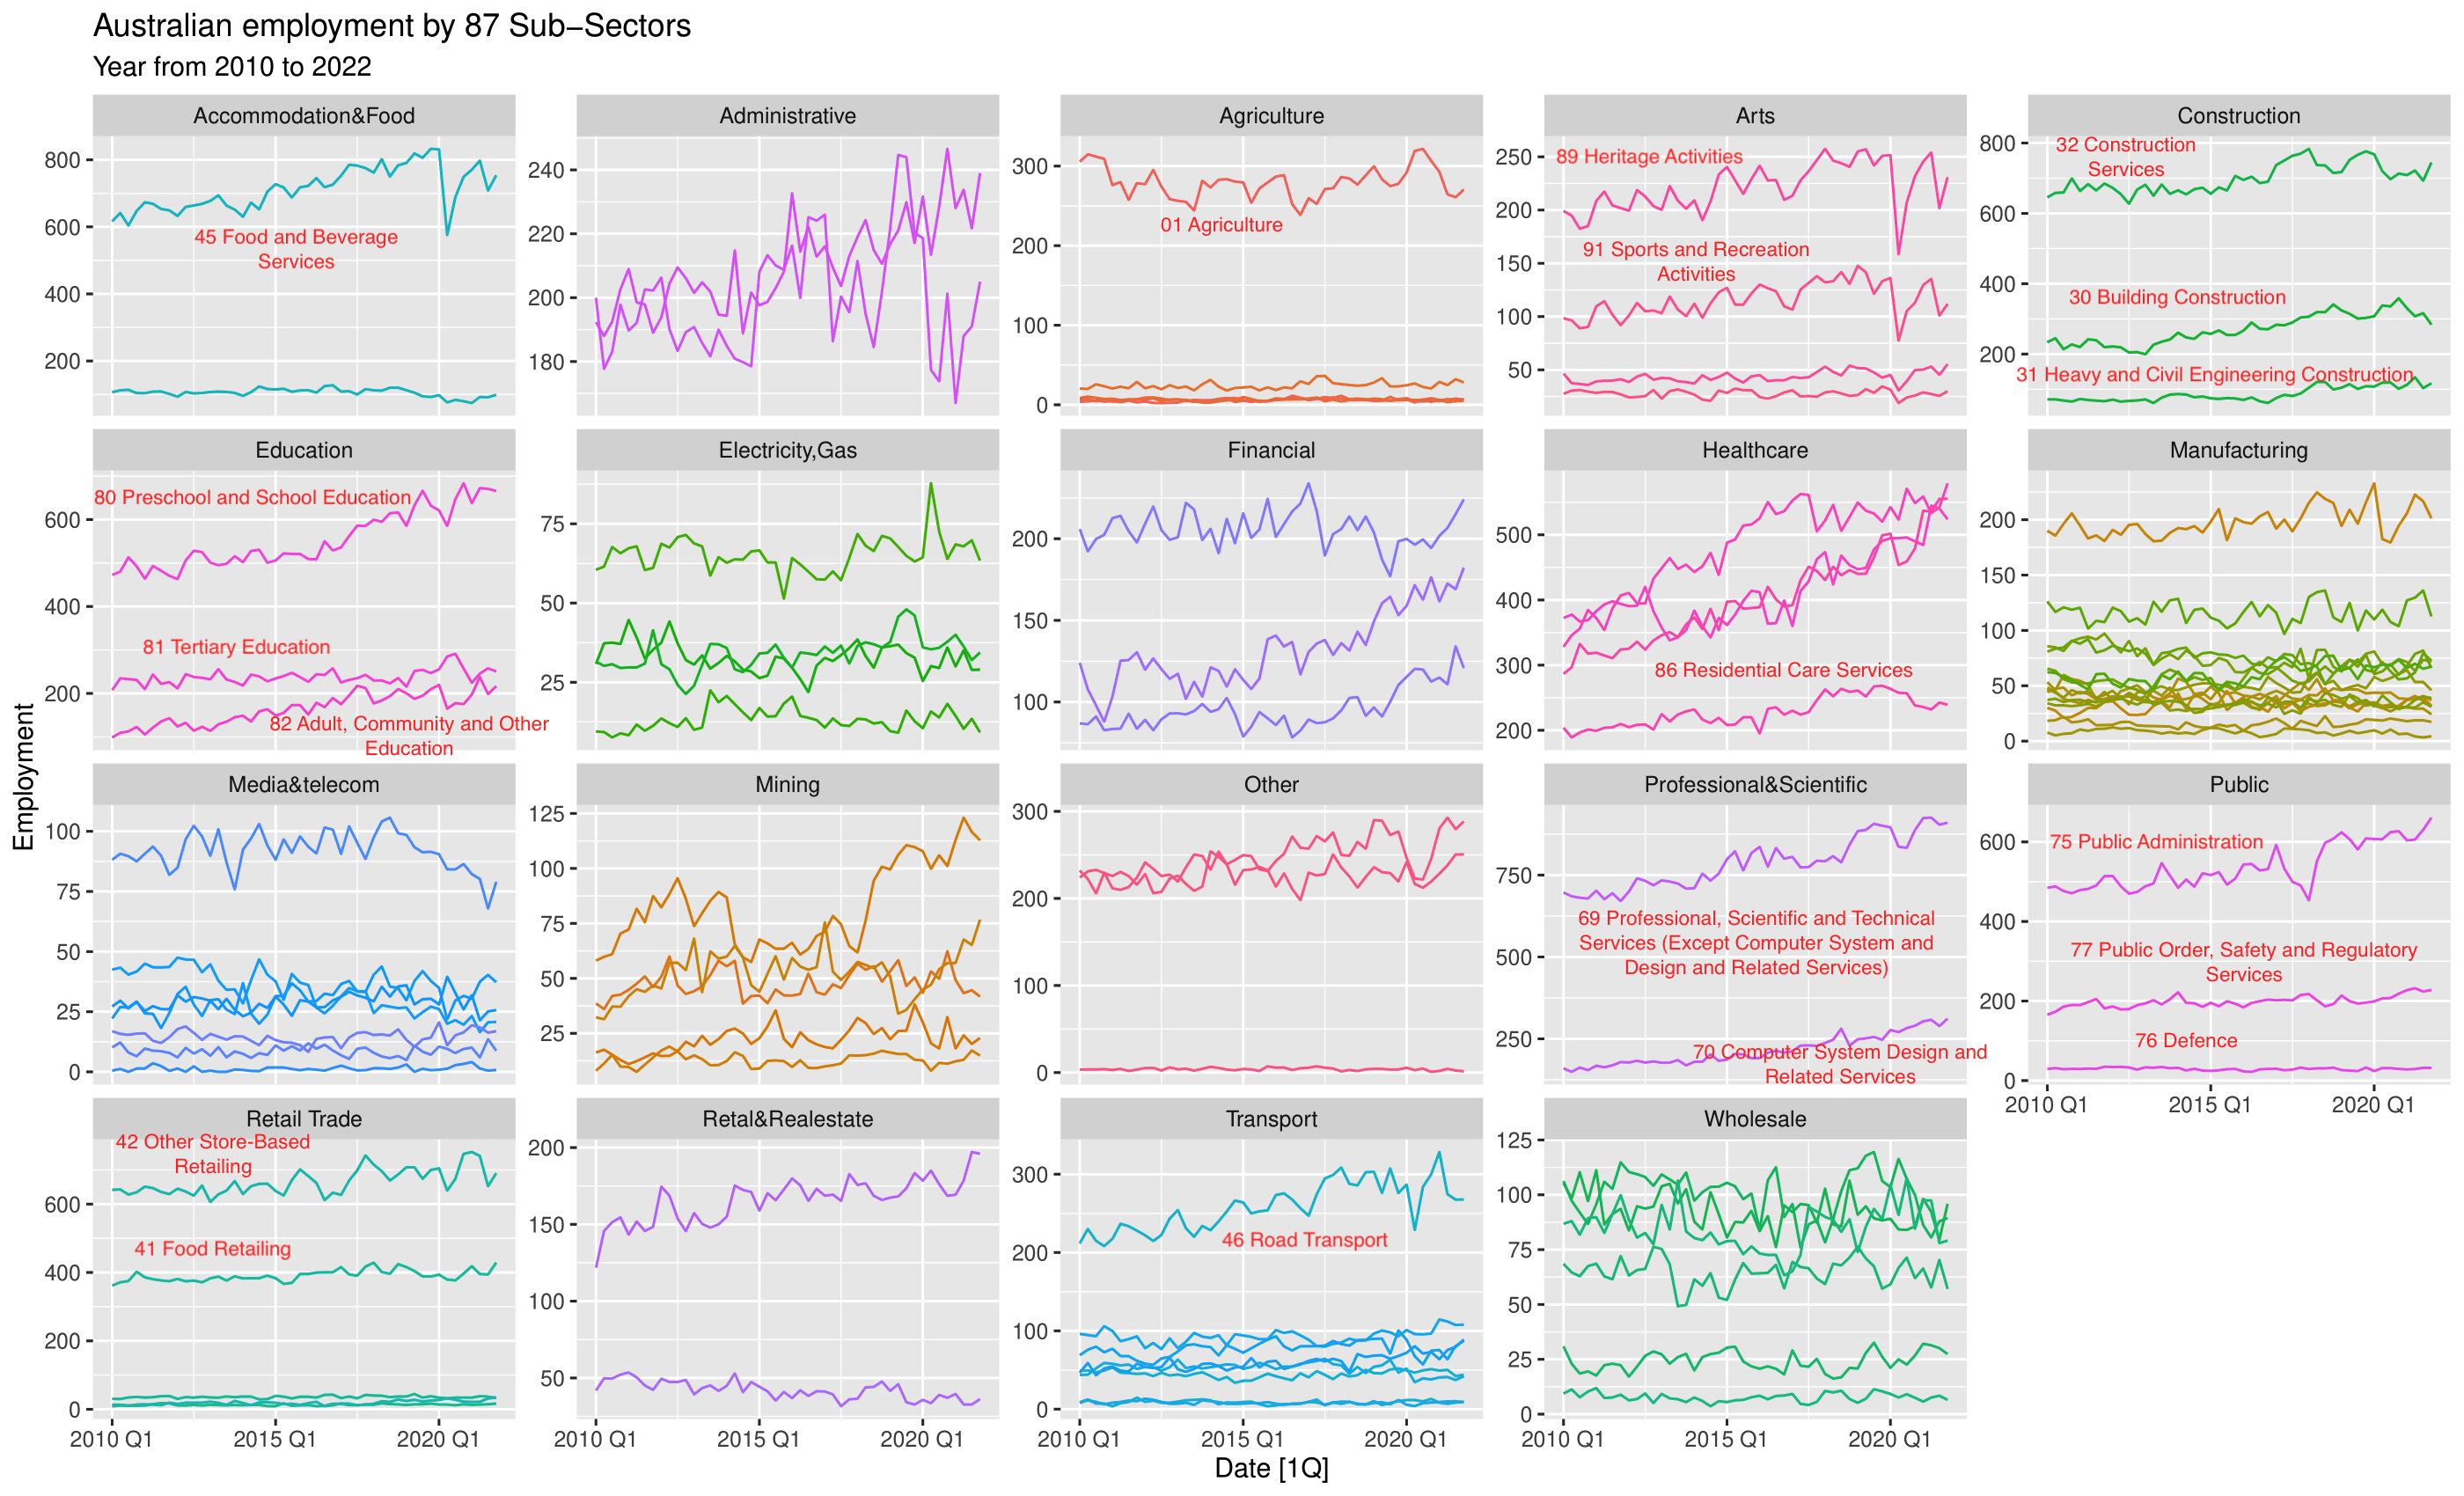
\includegraphics[scale=0.5]{87sec}
\centering
\caption{Employment('000) of two-digit subsectors in Australia from 2010 to 2022}
\label{fig:86}
\end{figure}

\begin{table}[ht]
  \centering
  \caption{\textbf{The long run Employment Multipliers Analysis (84 Disaggregated Sectors)} Sorted by Shares of Subsectors}
  \scalebox{0.5}{
    \begin{tabular}{|l|r|rrrr|rr|}
    \hline 
    Sub-Sector & Shares & 1 Year  & \multicolumn{1}{l}{2 Years } & \multicolumn{1}{l}{5 Years} & \multicolumn{1}{l}{10 Years } & M10/M0 & M10-M0 \\
    \hline\hline
  69 Professional, Scientific and Technical Services (Except Computer System) Design and Related Services) & 0.06931674 & 0.0485337 & 0.062318 & 0.06666942 & 0.06671967 & 0.96253315 & -0.0025971 \\
    45 Food and Beverage Services & 0.06348661 & 0.04693738 & 0.06311697 & 0.0666367 & 0.06668314 & 1.05034955 & 0.00319652 \\
    32 Construction Services & 0.05913525 & 0.04299346 & 0.05568259 & 0.05863971 & 0.05867338 & 0.99218952 & -0.0004619 \\
    42 Other Store-Based Retailing & 0.05378582 & 0.04963343 & 0.06655111 & 0.07145667 & 0.07151944 & 1.32970786 & 0.01773361 \\
    80 Preschool and School Education & 0.0492665 & 0.02091953 & 0.01855257 & 0.01721796 & 0.01720194 & 0.34916098 & -0.0320646 \\
    75 Public Administration & 0.04641708 & 0.01553789 & 0.01250828 & 0.01080403 & 0.01078435 & 0.23233592 & -0.0356327 \\
    85 Medical and Other Health Care Services & 0.04116996 & 0.02431334 & 0.02916687 & 0.02989798 & 0.02990662 & 0.72641828 & -0.0112633 \\
    84 Hospitals & 0.0369132 & 0.01785159 & 0.0199097 & 0.02042347 & 0.02042915 & 0.55343755 & -0.016484 \\
    87 Social Assistance Services & 0.03680509 & 0.02207106 & 0.02929537 & 0.0311832 & 0.03120476 & 0.84783798 & -0.0056003 \\
    41 Food Retailing & 0.03040546 & 0.01923095 & 0.02775936 & 0.03134743 & 0.0313965 & 1.03259348 & 0.00099102 \\
    30 Building Construction & 0.02365835 & 0.01966493 & 0.02362512 & 0.02432029 & 0.02432822 & 1.02831441 & 0.00066987 \\
    46 Road Transport & 0.02212746 & 0.01012106 & 0.01115604 & 0.01122802 & 0.011232 & 0.50760455 & -0.0108955 \\
    01 Agriculture & 0.02177417 & 0.00998719 & 0.01235378 & 0.01409829 & 0.01411674 & 0.64832471 & -0.0076574 \\
    95 Personal and other services (include activities for own use) & 0.02127031 & 0.0127474 & 0.01505848 & 0.01597865 & 0.01599074 & 0.75178666 & -0.0052796 \\
    86 Residential Care Services & 0.02028961 & 0.0108231 & 0.01516439 & 0.01583014 & 0.0158379 & 0.78059125 & -0.0044517 \\
    70 Computer System Design and Related Services & 0.01989965 & 0.01064273 & 0.01220485 & 0.0126649 & 0.01267126 & 0.63675763 & -0.0072284 \\
    81 Tertiary Education & 0.01945371 & 0.00166075 & -0.0015457 & -0.0021075 & -0.0021148 & -0.1087109 & -0.0215685 \\
    72 Administrative Services & 0.01790544 & 0.02068182 & 0.02911507 & 0.03127308 & 0.03129963 & 1.74805115 & 0.01339419 \\
    94 Repair and Maintenance & 0.0177703 & 0.01434611 & 0.02128838 & 0.02357418 & 0.0236012 & 1.32812526 & 0.00583089 \\
    73 Building Cleaning, Pest Control and Other Support Services & 0.01736876 & 0.01180556 & 0.01573853 & 0.01716652 & 0.01718243 & 0.98927169 & -0.0001863 \\
    11Food Product Manufacturing & 0.01649038 & 0.00702254 & 0.00846642 & 0.00827582 & 0.00827409 & 0.50175246 & -0.0082163 \\
    82 Adult, Community and Other Education & 0.01566605 & 0.00554203 & 0.00471415 & 0.00475267 & 0.00475016 & 0.30321348 & -0.0109159 \\
    77 Public Order, Safety and Regulatory Services & 0.01521818 & 0.00871417 & 0.01309719 & 0.01440524 & 0.01442184 & 0.94767203 & -0.0007963 \\
    62 Finance & 0.01472397 & 0.00857652 & 0.01062002 & 0.0110417 & 0.01104891 & 0.75040274 & -0.0036751 \\
    67 Property Operators and Real Estate Services & 0.01358111 & 0.00573538 & 0.00632144 & 0.00644085 & 0.00644122 & 0.47427795 & -0.0071399 \\
    64 Auxiliary Finance and Insurance Services & 0.01229925 & 0.00710233 & 0.00875331 & 0.00932324 & 0.00933078 & 0.75864648 & -0.0029685 \\
    91 Sports and Recreation Activities & 0.01027608 & 0.00887835 & 0.01209347 & 0.01274308 & 0.01275193 & 1.24093321 & 0.00247585 \\
    24Machinery and Equipment Manufacturing & 0.0087394 & 0.00384771 & 0.00486625 & 0.00522805 & 0.00523156 & 0.59861717 & -0.0035078 \\
    34 Machinery and Equipment Wholesaling & 0.00863129 & 0.00463038 & 0.00550646 & 0.00586781 & 0.00587311 & 0.68044432 & -0.0027582 \\
    39Motor Vehicle and Motor Vehicle Parts Retailing & 0.00844596 & 0.01088201 & 0.01646315 & 0.01809008 & 0.01810914 & 2.14411792 & 0.00966318 \\
    08 Metal Ore Mining & 0.00838419 & 0.00574686 & 0.00556897 & 0.0053132 & 0.00530956 & 0.6332827 & -0.0030746 \\
    31 Heavy and Civil Engineering Construction & 0.00832434 & 0.00731709 & 0.01027104 & 0.01102691 & 0.01103652 & 1.32581315 & 0.00271218 \\
    63 Insurance and Superannuation Funds & 0.00805214 & 0.00443011 & 0.00497832 & 0.00501181 & 0.00501281 & 0.62254327 & -0.0030393 \\
    51 Postal and Courier Pick-up and Delivery Services & 0.00757723 & 0.00121361 & 0.00131748 & 0.00140896 & 0.00141185 & 0.18632811 & -0.0061654 \\
    44 Accommodation & 0.00753476 & 0.0032441 & 0.00545 & 0.00634005 & 0.00635098 & 0.84289032 & -0.0011838 \\
    37 Other Goods Wholesaling & 0.0071892 & 0.00459914 & 0.00631193 & 0.00661623 & 0.00662058 & 0.92090624 & -0.0005686 \\
    58 Telecommunications Services & 0.00707916 & 0.00011311 & -0.001374 & -0.0014087 & -0.001411 & -0.1993137 & -0.0084901 \\
  33 Basic Material Wholesaling & 0.00697878 & 0.00828557 & 0.01222171 & 0.01343315 & 0.01344743 & 1.92690232 & 0.00646865 \\
    52 Transport Support Services & 0.00675677 & 0.00753772 & 0.01162295 & 0.01291333 & 0.01292955 & 1.91356851 & 0.00617277 \\
    21Primary Metal and Metal Product Manufacturing & 0.0058726 & 0.00462923 & 0.00499628 & 0.00494162 & 0.00494054 & 0.84128732 & -0.0009321 \\
    22Fabricated Metal Product Manufacturing & 0.00538804 & 0.0066765 & 0.00944416 & 0.01058564 & 0.01059958 & 1.96724154 & 0.00521154 \\
    53 Warehousing and Storage Services & 0.00527028 & 0.00263016 & 0.00272967 & 0.00287253 & 0.00287296 & 0.54512411 & -0.0023973 \\
    23Transport Equipment Manufacturing & 0.00514673 & 0.00299308 & 0.00469464 & 0.00556819 & 0.0055781 & 1.08381385 & 0.00043137 \\
    26Electricity Supply & 0.00502125 & 0.00491081 & 0.00586741 & 0.00563882 & 0.005636 & 1.12243022 & 0.00061475 \\
    25Furniture and Other Manufacturing & 0.00496526 & 0.00907029 & 0.01434533 & 0.01635773 & 0.01637974 & 3.29886584 & 0.01141447 \\
    36 Grocery, Liquor and Tobacco Product Wholesaling & 0.00491893 & 0.00061785 & -0.0006336 & -0.0008216 & -0.0008238 & -0.1674704 & -0.0057427 \\
    49 Air and Space Transport & 0.00419885 & 0.00350454 & 0.00513191 & 0.00542985 & 0.00543509 & 1.29442326 & 0.00123624 \\
    18 Basic Chemical and Chemical Product Manufacturing & 0.00395754 & 0.00606204 & 0.00950461 & 0.01069071 & 0.01070637 & 2.70531007 & 0.00674883 \\
    06 Coal Mining & 0.00383591 & 0.00383353 & 0.00407393 & 0.00408138 & 0.00408139 & 1.06399293 & 0.00024547 \\
    47 Rail Transport & 0.00381661 & 0.00126166 & 0.00105419 & 0.00112838 & 0.00112925 & 0.29587899 & -0.0026874 \\
    90 Creative and Performing Arts Activities & 0.00360425 & 0.00468914 & 0.00613651 & 0.00651375 & 0.00651912 & 1.80872881 & 0.00291486 \\
    14Wood Product Manufacturing & 0.00347877 & 0.00302624 & 0.00302602 & 0.00331986 & 0.00332296 & 0.9552116 & -0.0001558 \\
    29Waste Collection, Treatment and Disposal Services & 0.00339383 & 0.00565936 & 0.00756816 & 0.0078664 & 0.0078681 & 2.31835492 & 0.00447427 \\
    89 Heritage Activities & 0.00301159 & 0.00369792 & 0.0051636 & 0.00528106 & 0.00528232 & 1.7539992 & 0.00227074 \\
    10 Exploration and Other Mining Support Services & 0.00299228 & -0.0006873 & -0.0017035 & -0.0019049 & -0.0019072 & -0.6373821 & -0.0048995 \\
    55 Motion Picture and Sound Recording Activities & 0.00294209 & 0.00032963 & -0.0005498 & -0.0005605 & -0.0005605 & -0.1905091 & -0.0035026 \\
    40 Fuel Retailing & 0.00291506 & -0.0012046 & -0.0024966 & -0.0027078 & -0.0027087 & -0.9292227 & -0.0056238 \\
    66 Rental and Hiring Services (except Real Estate) & 0.00287066 & 0.003369 & 0.00341671 & 0.00336895 & 0.00336725 & 1.17298563 & 0.00049658 \\
    19Polymer Product and Rubber Product Manufacturing & 0.00283012 & 0.00233992 & 0.00331413 & 0.00359534 & 0.00359859 & 1.27153097 & 0.00076847 \\
    20Non-Metallic Mineral Product Manufacturing & 0.00277221 & 0.00357344 & 0.00319618 & 0.0030411 & 0.0030398 & 1.0965273 & 0.00026759 \\
    16Printing (including the Reproduction of Recorded Media) & 0.00262163 & -0.000264 & 0.00122375 & 0.00182629 & 0.00183417 & 0.69963121 & -0.0007875 \\
    12Beverage and Tobacco Product Manufacturing & 0.00252896 & 0.00277597 & 0.00231169 & 0.00223403 & 0.00223473 & 0.88365682 & -0.0002942 \\
    28Water Supply, Sewerage and Drainage Services & 0.00249614 & 0.00282008 & 0.00239868 & 0.00201716 & 0.0020111 & 0.80568129 & -0.000485 \\
    13Textile, Leather, Clothing and Footwear Manufacturing & 0.00244016 & 0.00487731 & 0.00773749 & 0.00862047 & 0.00863239 & 3.53763202 & 0.00619223 \\
    92 Gambling Activities & 0.00243437 & 0.00430809 & 0.00667533 & 0.00741282 & 0.00742126 & 3.04853477 & 0.00498689 \\
    07 Oil and Gas Extraction & 0.00232626 & -0.0017933 & -0.0034336 & -0.0039433 & -0.0039495 & -1.6977721 & -0.0062757 \\
    56 Broadcasting (except Internet) & 0.00225097 & 0.00562035 & 0.00883845 & 0.00960654 & 0.00961432 & 4.27118764 & 0.00736334 \\
    35 Motor Vehicle and Motor Vehicle Parts Wholesaling & 0.00208109 & 0.00130996 & 0.0019761 & 0.0022859 & 0.00228915 & 1.09997643 & 0.00020806 \\
    76 Defence & 0.00203668 & 0.00108328 & 0.00081797 & 0.00081458 & 0.00081483 & 0.40007524 & -0.0012219 \\
    05 Agriculture, Forestry and Fishing Support Services & 0.00201545 & 0.00410222 & 0.00612542 & 0.00684863 & 0.00685748 & 3.40246046 & 0.00484203 \\
    54 Publishing and Broadcasting & 0.00199035 & 0.00146161 & 0.00254755 & 0.00299741 & 0.00300331 & 1.50893341 & 0.00101296 \\
    43 Non-Store Retailing and Retail Commission Based Buying and/or Selling & 0.00198842 & 0.00008765 & -0.0006368 & -0.0010072 & -0.0010108 & -0.5083429 & -0.0029992 \\
    15Pulp, Paper and Converted Paper Product Manufacturing & 0.00134556 & 0.00088098 & 0.00127857 & 0.00145108 & 0.00145231 & 1.07933418 & 0.00010675 \\
    60 Library and Other Information Services & 0.00113321 & 0.00262681 & 0.00408402 & 0.00438669 & 0.00438973 & 3.8737221 & 0.00325652 \\
    09 Non-Metallic Mineral Mining and Quarrying & 0.00109846 & 0.00030124 & 0.00035283 & 0.00047586 & 0.00047618 & 0.43350017 & -0.0006223 \\
    27Gas Supply & 0.00093436 & 0.00119372 & 0.00200704 & 0.00226239 & 0.00226542 & 2.42456061 & 0.00133106 \\
    38 Commission-Based Wholesaling & 0.00073359 & 0.00117105 & 0.00148834 & 0.00157279 & 0.00157404 & 2.14566446 & 0.00084045 \\
    59 Internet Service Providers, Web Search Portals and Data Processing Services & 0.00071236 & -0.0002143 & -0.0006387 & -0.0006332 & -0.0006331 & -0.8887063 & -0.0013454 \\
    48 Water Transport & 0.00067182 & -0.0003845 & -0.0003261 & -0.0002884 & -0.0002886 & -0.4295098 & -0.0009604 \\
    17Petroleum and Coal Product Manufacturing & 0.00066795 & 0.00026082 & -0.0002759 & -0.0005609 & -0.0005649 & -0.8457507 & -0.0012329 \\
    50 Other Transport & 0.00062162 & 0.00128362 & 0.00155246 & 0.00160919 & 0.00160982 & 2.58970933 & 0.0009882 \\
    03 Forestry and Logging & 0.00053668 & -0.0012108 & -0.0017314 & -0.0018066 & -0.0018077 & -3.3683565 & -0.0023444 \\
    02 Aquaculture & 0.00050193 & -0.0001496 & -0.0003808 & -0.0004863 & -0.0004873 & -0.9709079 & -0.0009893 \\
    04 Fishing, Hunting and Trapping & 0.00046139 & 0.00209291 & 0.00329398 & 0.00352863 & 0.00353112 & 7.65320735 & 0.00306973 \\
    \hline\hline 
    \end{tabular}} 
    \begin{tablenotes} 
      \footnotesize
      \item \emph{Note}: The long run employment multiplier for subsector $i$ is the effect of a 1\% increase in employment of subsector on total employment in the long run. \\
      M10 is the long term multiplier; M0 is the share of subsector $i$ in total employment.
      M10-M0 is the spillover of the subsector $i$. \\
      M10/M0 is the spillover of the subsector $i$ relative to the share of it.
\end{tablenotes}
\caption{Disaggregated Sectoral Long-Run Employment Multipliers: Full list of 84 sectors (Sorted by Shares)}
  \label{dis:emp}
\end{table}

\hypertarget{supplementary-materials-data-codes}{%
\chapter{Supplementary Materials (Data \& Codes)}\label{supplementary-materials-data-codes}}

Supplementary materials include figures, codes and documentations can be found in the Github repo of this project: {[}Link: \url{https://github.com/elvisssyang/Disaggregated_Employment}{]}. Please contact me via Github or email me at \texttt{zyan0056@student.monash.edu} if something is unclear.

\printbibliography[heading=bibintoc]



\end{document}
